% don't remove the following lines, and edit the definition of \main if needed
\documentclass[../report.tex]{subfiles}
\providecommand{\main}{..}
\IfEq{\jobname}{\currfilebase}{\AtEndDocument{\biblio}}{}
% until here

%file for shortcuts

\newcommand{\nch}{\ensuremath{N_{\mathrm {ch}}\xspace}}
\newcommand{\Ncoll}{\ensuremath{N_{\mathrm {coll}}}}
\newcommand{\Npart}{\ensuremath{N_{\mathrm {part}}}}
\newcommand{\dNdeta}{\mathrm{d}N_\mathrm{ch}/\mathrm{d}\eta}
\newcommand{\snn}         {\ensuremath{\sqrt{s_{\mathrm {NN}}}}}
\newcommand{\kT}          {\ensuremath{k_{\mathrm {T}}}}

\newcommand{\pp}          {pp}
\newcommand{\pPb}         {pPb}
\newcommand{\pA}          {pA}
\newcommand{\PbPb}        {PbPb}
\newcommand{\AuAu}        {AuAu}
\newcommand{\CuCu}        {CuCu}
\newcommand{\pAu}         {pAu}
\newcommand{\dAu}         {dAu}
\newcommand{\lsim}        {\,{\buildrel < \over {_\sim}}\,}
\newcommand{\gsim}        {\,{\buildrel > \over {_\sim}}\,}
\newcommand{\co}[1]       {\relax}
\newcommand{\nl}          {\newline}
\newcommand{\el}          {\\\hline\\[-0.4cm]}

\emergencystretch=1em
\raggedbottom

\begin{document}

\section{Emergence of Hot and Dense QCD in Small Systems}
In the program of proton-proton collisions at the LHC, the main effort is focused in hard processes which are embedded in an 
underlying event consisting of a large number of soft low-$p_\perp$ particles. The underlying event is subtracted using models, such as PYTHIA \cite{Sjostrand:2014zea} or HERWIG \cite{Bellm:2015jjp}, based on essentially free streaming of the produced particles, supplemented in some cases with a non-perturbative string fragmentation picture \cite{Andersson:1983ia} to model the non-perturbative soft particle production.  

In the past years at LHC, during run 1 and 2, this picture was challenged by the several observations that qualitatively differ from the model expectations and can not be accommodated by tuning of the existing models used to describe the underlying event \cite{Fischer:2016zzs}.
The first such observation was the unexpected discovery of azimuthal correlations of final state hadrons that persist even at large separations in rapidity, originally seen by the CMS collaboration in proton-lead collisions. Qualitatively similar, but quantitatively smaller, signal was subsequently observed also in proton-proton collisions extending from high multiplicities (N > 110) down to minimum bias events. The second observation was that of enhanced production of multi-strange hadrons in high-multiplicity proton-proton collisions extending the discrepancy from final state particle kinematics to include also hadrochemistry. 

In ultrarelativistic nucleus-nucleus collisions, ranging from early SPS experiment at CERN through Relativistic Heavy-Ion Collider (RHIC) at Brookhaven National Laboratory (BNL) to LHC, these qualitative observations have been have been interpreted as signs of formation of a droplet of thermalized quark-gluon plasma. The long range azimuthal correlations, and in particular their lowest harmonic components $v_2$, have been used in combination with relativistic fluid-dynamical modeling to constrain the material properties of the plasma.  The striking result from RHIC was that the plasma formed in the central nucleus-nucleus (Au-Au) collisions flows as a liquid nearly without dissipation such that its specific viscosity $\eta/s$ -- quantifying the dissipative properties of the medium -- was found to be smaller than that of any other known substance. The inferred value of the specific shear viscosity $\eta/s\sim 0.07-0.16$ \cite{} was found to be significantly smaller than the expectation from perturbative QCD and other quasiparticles models and closer to the expectation of holographic model calculations of strongly coupled (maximally supersymmetric N=4) gauge theories in the limit of large number of colors $N_c \rightarrow \infty$. These models can be seen as models of fluids with minimal dissipation allowed by basic principles of  quantum mechanics thus giving rise to the paradigm of quark-gluon plasma as a perfect liquid. The models of perfect fluid do not have a quasiparticle structure, and as such they are incompatible with free streaming. Therefore, the observation of fluid-like signatures as a small modification of free streaming evolution in small systems also challenges the perfect fluid paradigm. 

There are several theoretical pictures that have been suggested to explain the smooth onset of signals of collectivity in small systems. The pp event generators have been supplemented on one hand with elements describing string fragmentation in dense medium (DIPSY) to address the hadrochemisty and on other hand final state interactions between the fragmenting strings to account for the final state kinematical correlations \cite{Bierlich:2017vhg}. 
The models of perfect fluid have been brought to their extreme and applied down to proton-proton collisions \cite{Weller:2017tsr,Aidala:2018mcw} suggesting a formation of nearly perfect liquid even in the smallest collision systems. Furthermore pQCD based saturation models can describe emergence of $v_2$. In these models the final state azimuthal correlations can arise either from the intrinsic correlations in the nuclear wave function (initial state correlations) as correlated anisotropic particle production or as a final state interaction after the initial particle production. 
A question remains to what extent these different models are describing qualitatively different physical phenomena or to what extent they are different prescriptions of the same underlying physics of final state interactions. Transport theory, which can describe microscopic interactions but in the limit of large number of final state interactions has a coarse grained effective description in terms of fluid dynamics has the potential to bridge the gap between the small systems where final state interactions act as small modification to free streaming evolution and the central nucleus-nucleus collisions where the final state interactions bring the matter to the fluid dynamical limit. 

The experimental program in the large intermediate region --- spanning from mid-central Pb-Pb and Xe-Xe, through p-A down to min-bias pp collisions (and possibly even very high multiplicity e+e- and e-p events) --- offers a possibility to reconcile the difference in the two limits by proving a setup where the microscopic final state interactions that lead in central PbPb collision to the formation of QGP may be studied in isolation in the limit of small number of final state interactions.  

The suggested theoretical pictures also possibly have implications for high energy physics analyses, which depend on reliable models of the underlying event. As an example, the ATLAS collaboration have recently shown the appearance of a ridge in the underlying event of $Z$-tagged pp collisions. As the usual models used to describe the underlying event fails, even qualitatively, to describe this, better descriptions of collective effects in small systems are also vital for improving understanding even in high energy analyses.


\subsection{Historic overview}
% Comments wrt initial LHC program

In recent years, LHC experiments have measured different observables in Pb--Pb collisions. Some of these observables have been also measured in smaller systems such as high multiplicity proton-proton and proton-lead collisions. In order to understand these phenomena in different collision systems the observed phenomena are classified in different groups. The $p_{\rm{T}}$-spectra of almost all particles are described by hydrodynamic models at low $p_{\rm{T}}$ values ($p_{\rm{T}} < 2 $ GeV/$c$) \cite{Abelev:2012wca,Abelev:2013vea,Chatrchyan:2013eya,Chatrchyan:2012qb,Andrei:2014vaa,Abelev:2013haa,Acharya:2017dmc,Adam:2016bpr,Adam:2015vsf,Adam:2017zbf}. Hydrodynamic models translate initial spatial anisotropies ($\varepsilon_n$) into final momentum anisotropies, namely anisotropic flow ($v_{n}$) assuming that the pressure gradients build up early in the evolution of the system. Hydrodynamic models have been able to describe the average radial velocity or radial flow in all collision systems. In addition, several measurements have been done on the anisotropic flow harmonics. Higher flow harmonics are more sensitive to initial state fluctuations and therefore can constrain the initial conditions of the system. Due to this several measurements have been done in LHC experiments and more efforts are on the way to reach even higher flow harmonics. Up until this moment, anisotropic flow has been measured with two particle correlation techniques up to $v_7$ in Pb--Pb collisions, $v_5$ in pPb and $v_4$ in pp collisions for charged particles \cite{CMS:2012qk,Abelev:2012ola,Aad:2012gla,Aamodt:2011by,Chatrchyan:2011eka,Chatrchyan:2012wg,ATLAS:2012at,Aad:2014lta,Aad:2015gqa,CMS:2015zpa,Khachatryan:2016txc,Acharya:2017ino,Adam:2016ows,Adam:2016nfo,Acharya:2018zuq,Sirunyan:2017uyl,Aaboud:2017acw}.

Higher order cumulants have been measured up to 8 particle correlations for both Pb--Pb and pPb collisions and up to 6 particle correlations for pp collisions \cite{Aad:2013fja,Chatrchyan:2013nka,Khachatryan:2016txc,Aamodt:2010pa,ALICE:2011ab,Chatrchyan:2012ta,Abelev:2014mda,Chatrchyan:2013kba,Aad:2014vba,Khachatryan:2015waa,Adam:2016izf,CMS:2015ica,Sirunyan:2017pan,Sirunyan:2017igb,Aaboud:2017acw,Aaboud:2017blb}. Interestingly, for each collision system, the measurements of the cumulants with different higher order particle correlations ($n \geq 4$) are similar within 10\%. Presence of non-zero higher-order cumulants with similar magnitude could be interpreted as an evidence for a hydrodynamically evolving system. However, some disfavor this interpretation since models that do not incorporate hydrodynamics have been able to predict these results. The $p_{\rm{T}}$-differential $v_{n}$ measurements for identified particles present the characteristic mass dependence of anisotropic flow up to $v_{5}$ in Pb--Pb collisions $v_{3}$ in pPb and $v_{2}$ in pp collisions \cite{Abelev:2014pua,Abelev:2012di,Adam:2016nfo,Khachatryan:2014jra,ABELEV:2013wsa,CMS:2015kua,Khachatryan:2016txc,Acharya:2018zuq}. This mass dependence has been described by hydrodynamic calculations to a good approximation in all three systems.

Recently, both linear and non-linear hydrodynamic response of the system produced in Pb--Pb collisions have been investigated up to the sixth harmonic for both charged and identified particles where hydrodynamic calculations show promising predictions in low $p_{\rm{T}}$ values which help constraining the transport properties of the QGP created in Pb--Pb collisions \cite{Acharya:2017zfg}. Linear and non-linear flow modes in pp and pPb collisions are yet to be measured. Such measurements help constraining the transport properties as well as initial conditions of these small systems. Furthermore, hydrodynamic calculations capture '"higher order" details (at least qualitatively), such as the breaking of factorization due to event-plane angle decorrelations in $p_{\rm{T}}$ and $\eta$ measured in both Pb--Pb and pPb collisions \cite{Khachatryan:2015oea,Sirunyan:2017gyb,Acharya:2017ino} and yet to be measured in pp collisions. Hydrodynamic calculations can be tested in event-by-event $v_{n}$ distributions as well as event-plane angle and $v_{n}$ correlations across different harmonics \cite{Aad:2014fla,Aad:2015lwa,ALICE:2016kpq,Sirunyan:2017uyl}. So far event-by-event $v_{n}$ measurements have only been done in Pb--Pb collisions \cite{Aad:2013xma,Sirunyan:2017fts} and it needs to be investigated in both pPb and pp collisions. 

Directed flow, both the rapidity-odd as well as the rapidity-even components, of charged particles at mid-rapidity was measured relative to the collision symmetry plane defined by the spectator nucleons, and evidence for dipole-like initial density fluctuations in the overlap region was found in Pb--Pb collisions \cite{Abelev:2013cva}. Charge dependent azimuthal correlations are also measured in both Pb--Pb and pPb collisions which indicates a local parity and CP violation \cite{Adam:2015vje,Sirunyan:2017tax,Acharya:2017fau,Sirunyan:2017quh,Khachatryan:2016got}. In small systems, the concept of directed flow is not very clear specially in pp collisions. If there is collectivity in pp collisions one could also expect a non-zero directed flow measurement. Since no spectator plane is expected in small systems, $v_{1}$ could only be calculated using higher order ($n\geq 4$) cumulants. However, charge dependent $v_{1}$ could not be expected as there is no spectator plane to create a magnetic field in the system. 

In the intermediate $p_{\rm{T}}$ values ($2 < p_{\rm{T}} < 5 $ GeV/$c$), particle yields present larger magnitudes for heavier particles which is described by quark coalescence as the main particle production mechanism, combined with hydrodynamics. This effect that is usually referred to as recombination is present in all three systems \cite{Andrei:2014vaa,Abelev:2013xaa,Abelev:2013haa,Abelev:2014uua,Khachatryan:2016yru,Adam:2015jca,Adam:2016dau,Adam:2017zbf}. Particle ratios and yields are described as a Grand Canonical ensemble by the statistical model with the strangeness undersaturation factor $\rm{Y}_{S}\approx 1$ at an approximate level of 10-30\% for a Pb--Pb collision and 20-40\% for pPb collisions (except for the $\Omega$ meson). The statistical model has been so far applied to the minimum bias pp collisions and when treated as a canonical ensemble, was found to describe the yields with $\rm{Y}^{C}_{S} < 1$ and deviations of only about 20-40\% from the expected yields \cite{Adam:2016emw,Adam:2016bpr,Adam:2015vsf,ABELEV:2013zaa}. 

The freeze-out radii in 3 orthogonal directions ("out", "side", "long") can be deduced from measurements of quantum-statistics correlations between pairs of same-charge pions and kaons (HBT) at low momentum transfer. The HBT radii in all collision systems are found to scale with 3 $N_{ch}$ (indicating a constant density at freeze-out) and to decrease with increasing pair momentum ($k_{\rm{T}}$) as expected from hydrodynamics. The size along the emission direction is similar to the geometric size of the system ($R_{out}/R_{side} \approx 1$) in Pb--Pb collisions and $R_{out}/R_{side} \leq 1$ for both pPb and pp collisions \cite{Adam:2015vna,Adam:2015vja,Abelev:2014pja,Adam:2015pya,Aamodt:2011kd,CMS:2014mla,ATLAS:2015-054,Acharya:2017qtq,Aaboud:2017xpw}.

Direct photon measurements at low $p_{\rm{T}}$ region are so far done in Pb--Pb and pp collisions and can be described approximately by hydrodynamic models. These models determine the initial temperature of the QGP produced in Pb--Pb collisions to exceed about 400 MeV in central collisions \cite{Adam:2015lda}. No significant direct photon signal has be extracted in pp collisions at current available center-of-mass energies \cite{Acharya:2018dqe}. The created system in Pb--Pb collisions is opaque for high-$p_{\rm{T}}$ colored probes and due to radiational and collisional energy loss (jet quenching) high-$p_{\rm{T}}$ colored probes are strongly suppressed whereas the system is transparent for photons and other colorless probes. Jet quenching leads to slightly modified jet fragmentation functions inside small jet cone sizes (R = 0.4), and most of the radiated energy appears at large angles (R > 0.8). Direct jet quenching has not been observed in small systems \cite{Aad:2010bu,Aamodt:2010jd,Chatrchyan:2011sx,CMS:2012aa,Abelev:2012hxa,ALICE:2012ab,Aad:2014bxa,Adam:2015ewa,Aad:2015wga,Adam:2016jfp,Adam:2016xbp,Sirunyan:2017jic,Sirunyan:2016fcs,Sirunyan:2018jqr,Sirunyan:2018jju,Sirunyan:2018qec,Sirunyan:2017qhf,Khachatryan:2016tfj,Sirunyan:2017bsd,Aaboud:2017bzv,Aaboud:2017eww}. 

Due to interactions and rescattering with the medium, even heavy-flavor particles exhibit finite anisotropies as shown with non-zero $v_{2}$ measurements for heavy flavour particles in both Pb--Pb and pPb collisions \cite{ALICE:2013xna,Abelev:2013lca,Abelev:2014ipa,Adam:2015pga,Acharya:2017tfn,Adam:2016ssk,ALICE:2016clc,Acharya:2017qps,Sirunyan:2017plt,Acharya:2017tgv,Khachatryan:2016ypw,Acharya:2018dxy,Sirunyan:2018toe}. Strong support for the formation of a deconfined medium with color degrees of freedom is the relative enhancement of J/$\psi$ yields, in particular at low $p_{\rm{T}}$, due to statistical recombination or regeneration, and the sequential suppression of $\rm{Y}$ states in Pb--Pb collisions. In pPb collisions, J/$\psi$ is suppressed relative to pp collisions \cite{Abelev:2012rv,Adam:2015rba,Chatrchyan:2012lxa, Chatrchyan:2013nza, Abelev:2014zpa, Adam:2015jsa, Adam:2016ohd, Adam:2015rta, Adam:2015isa, Adam:2015gba, Adam:2016rdg, Adamova:2017uhu, Acharya:2017tfn, Acharya:2017hjh, Sirunyan:2017lzi, Khachatryan:2016ypw, Sirunyan:2017mzd, Sirunyan:2017isk, Khachatryan:2016xxp, Sirunyan:2016znt, Aaboud:2017cif, Aaij:2017cqq}. 




% Table (-> Constantin, Naghmeh)

\begin{table}[h!]
\begin{center}
  \small
  \begin{tabular}{p{3.9cm}|p{2.7cm}|p{2.7cm}|p{2.6cm}| p{1.7cm} }
    Observable or effect                 & PbPb                                          & pPb (high mult.)                  & pp (high mult.)                         & Refs.\\
    \hline
    \hline
    Low $\pT$ spectra (``radial flow'')  & yes                                             & yes                                & yes                            & \cite{Abelev:2012wca,Abelev:2013vea,Chatrchyan:2013eya,Chatrchyan:2012qb,Andrei:2014vaa,Abelev:2013haa,Acharya:2017dmc,Adam:2016bpr,Adam:2015vsf,Adam:2017zbf} \el
    Intermed.\ $\pT$ (``recombination'') & yes                                             & yes                                & yes                            & \cite{Andrei:2014vaa,Abelev:2013xaa,Abelev:2013haa,Abelev:2014uua,Khachatryan:2016yru,Adam:2015jca,Adam:2016dau,Adam:2017zbf} \el
    Particle ratios                      & GC level                                        & GC level except $\Omega$           & GC level except $\Omega$       & \cite{Adam:2016emw,Adam:2016bpr,Adam:2015vsf,ABELEV:2013zaa} \\
    Statistical model                    & $\gamma^{\rm GC}_s=1$, 10--30\%                   & $\gamma^{\rm GC}_s\approx1$, 20--40\%  & $\gamma^{\rm C}_s<1$, 20--40\%  & \cite{Floris:2014pta,Adam:2015vsf,ALICE:2017jyt} \el
        HBT radii ($R(\kT)$, $R(\sqrt[3]{\nch})$)        & $R_{\mathrm{out}}/R_{\rm side}\approx1$& $R_{\rm out}/R_{\rm side}\lsim1$         & $R_{\rm out}/R_{\rm side}\lsim1$       & \cite{Adam:2015vna,Adam:2015vja,Abelev:2014pja,Adam:2015pya,Aamodt:2011kd,CMS:2014mla,Aaboud:2017xpw,Acharya:2017qtq,Aaboud:2017xpw} \el
       Azimuthal anisotropy ($v_n$)\nl 
    (from two part.\ correlations)                   & $v_{1}-v_{7}$                                 & $v_{1}-v_{5}$                                  & $v_{2}-v_{4}$                  & \cite{CMS:2012qk,Abelev:2012ola,Aad:2012gla,Aamodt:2011by,Chatrchyan:2011eka,Chatrchyan:2012wg,ATLAS:2012at,Aad:2014lta,Aad:2015gqa,CMS:2015zpa,Khachatryan:2016txc,Acharya:2017ino,Adam:2016ows,Adam:2016nfo,Acharya:2018zuq,Sirunyan:2017uyl,Aaboud:2017acw} \el                      
            Characteristic mass dependence                   & $v_2$ -- $v_5$            & $v_2$, $v_3$                               & $v_2$                         & \cite{Abelev:2014pua,Abelev:2012di,Adam:2016nfo,Khachatryan:2014jra,ABELEV:2013wsa,CMS:2015kua,Khachatryan:2016txc,Acharya:2018zuq} \el        
    Directed flow (from spectators)                  & yes                                       & no                                        & no                            & \cite{Abelev:2013cva}\el
        Charge dependent azimuthal correlations (CME, CMW)                   & yes                                       & yes                                       & not measured                            & \cite{Adam:2015vje,Sirunyan:2017tax,Acharya:2017fau,Sirunyan:2017quh,Khachatryan:2016got}\el
    Higher order cumulants \nl(mainly $v_2\{n\}$, $n\ge4$)  & \mbox{``$4\approx6\approx8\approx$ LYZ''} \mbox{+higher harmonics}&\mbox{``$4\approx6\approx8\approx$ LYZ''} \mbox{+higher harmonics}  & \mbox{``$4\approx6$''}  & \cite{Aad:2013fja,Chatrchyan:2013nka,Khachatryan:2016txc,Aamodt:2010pa,ALICE:2011ab,Chatrchyan:2012ta,Abelev:2014mda,Chatrchyan:2013kba,Aad:2014vba,Khachatryan:2015waa,Adam:2016izf,CMS:2015ica,Sirunyan:2017pan,Sirunyan:2017igb,Aaboud:2017acw,Aaboud:2017blb} \el
  Linear and non-linear \nl flow modes & yes (up to $v_{6}$) & no & no & \cite{Acharya:2017zfg} \el
    
  Weak $\eta$ dependence                           & yes                                       & yes                                       & not measured                  & \cite{Adam:2016ows,Aad:2014eoa,ATLAS:2011ah,Khachatryan:2016ibd,Adam:2015bka,Aaij:2015qcq,CMS:2015ica,Aaboud:2016jnr,Sirunyan:2017igb,Aaboud:2017tql} \el 
    Factorization breaking                           & yes ($n=2,3$)                             & yes ($n=2,3$)                             & not measured                  & \cite{Khachatryan:2015oea,Sirunyan:2017gyb,Acharya:2017ino}\el
    Event-by-event $v_n$ distributions               & $n=2-4$                                   & not measured                              & not measured                  & \cite{Aad:2013xma,Sirunyan:2017fts} \el
    Event plane and $v_n$ correlations               & yes                                       & yes                              & yes                  & \cite{Aad:2014fla,Aad:2015lwa,ALICE:2016kpq,Sirunyan:2017uyl} \el
   Direct photons at low $\pT$                      & yes                                       & not measured                              & yes  & \cite{Adam:2015lda,Acharya:2018dqe}\el
   Jet quenching                                    & yes                                       & not observed             & not observed  & \cite{Aad:2010bu,Aamodt:2010jd,Chatrchyan:2011sx,CMS:2012aa,Abelev:2012hxa,ALICE:2012ab,Aad:2014bxa,Adam:2015ewa,Aad:2015wga,Adam:2016jfp,Adam:2016xbp,Sirunyan:2017jic,Sirunyan:2016fcs,Sirunyan:2018jqr,Sirunyan:2018jju,Sirunyan:2018qec,Sirunyan:2017qhf,Khachatryan:2016tfj,Sirunyan:2017bsd,Aaboud:2017bzv,Aaboud:2017eww}\el
      Heavy flavor anisotropy                         & yes                                       & yes \cite{Acharya:2017tfn,Acharya:2018dxy,Sirunyan:2018toe}                       & not measured                   & \cite{ALICE:2013xna,Abelev:2013lca,Abelev:2014ipa,Adam:2015pga,Acharya:2017tfn,Adam:2016ssk,ALICE:2016clc,Acharya:2017qps,Sirunyan:2017plt,Acharya:2017tgv,Khachatryan:2016ypw,Acharya:2018dxy,Sirunyan:2018toe}\el
   Quarkonia                                        & J/$\psi \uparrow$, $\Upsilon \downarrow$  & suppressed                                & not measured & \cite{Abelev:2012rv,Adam:2015rba,Chatrchyan:2012lxa, Chatrchyan:2013nza, Abelev:2014zpa, Adam:2015jsa, Adam:2016ohd, Adam:2015rta, Adam:2015isa, Adam:2015gba, Adam:2016rdg, Adamova:2017uhu, Acharya:2017tfn, Acharya:2017hjh, Sirunyan:2017lzi, Khachatryan:2016ypw, Sirunyan:2017mzd, Sirunyan:2017isk, Khachatryan:2016xxp, Sirunyan:2016znt, Aaboud:2017cif, Aaij:2017cqq} \\

           
   \hline
    \hline
  \end{tabular}
  \caption{Summary of bulk observables or effects (classified as known from AA data) in PbPb collisions, as well as in high multiplicity pPb and pp collisions at the LHC. References to key measurements for the various observables and systems are given. See text for details.}
\end{center}  
\end{table}

\subsection{Open questions and their theoretical implications}

% Nature of collectivity / initial vs final state
% Are “collective effects” caused by final-state interactions in pp and pPb? → we should see jet quenching and medium-quark interactions
%   RAA, X+jet correlations
%   HF vn, Strangeness enhancement
% (Smooth?) transition from pp to pPb to PbPb
% Is there a turn on of at low Nch?
%   Subevents
%   Higher order cn (may be hopeless..)
% Make clear why pp and pPb are needed
% Integrate different modelling approaches (hydro, CGC, escape, …) 
% Shortcomings of current modelling in small systems (need to argue how run 3 and 4 can improve this)

\subsection{Key observables}

\subsubsection{Multiplicity distribution in pp}

For the performance estimates at high multiplicity in pp, a multiplicity-distribution extrapolation has been used which is based on existing ALICE ($|\eta| < 1.5$) \cite{Adam:2015gka} and ATLAS ($|\eta|< 2.5$) \cite{Aad:2010ac,Aad:2016xww} data. Data from CMS \cite{Khachatryan:2010nk} is compatible with the used distribution and is therefore not explicitly included in the extrapolation. A parameterisation with a single\footnote{At LHC energies two NBDs are needed for a good fit to the full distribution, but one is sufficient for the tail of the distribution.} negative binomial distribution is used which also have been frequently used to characterize the multiplicity distribution~\cite{GrosseOetringhaus:2009kz,ALICE:2017pcy}.

The data used is shown in Fig.~\ref{fig:smallsystems_mult_data}. The fit with a single negative binomial distribution of the tail of the distribution (20--40\% of the cross-section) is also shown. The three parameters of this fit are fit with a power-law fit to extrapolate to 14 TeV.

\begin{figure}[ht]
\centering
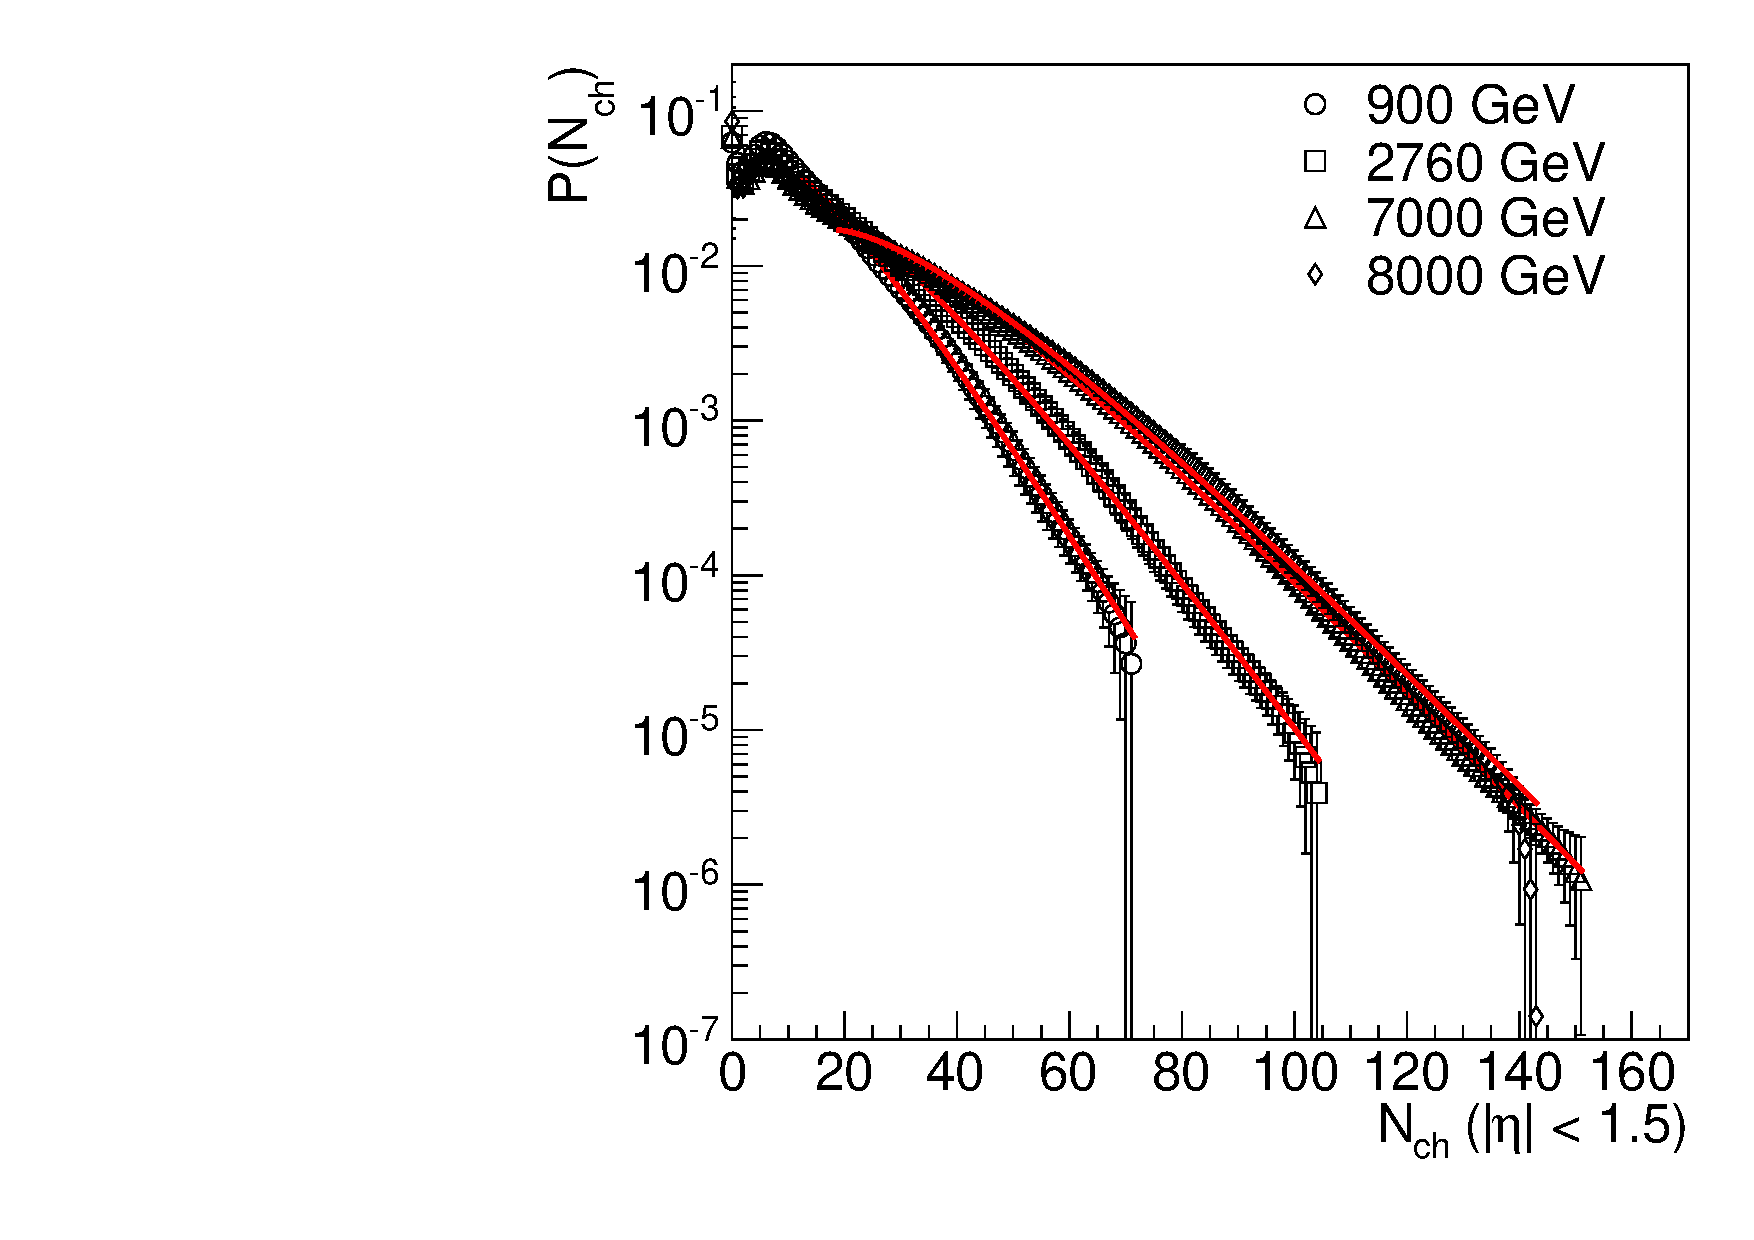
\includegraphics[width=0.49\linewidth]{\main/smallsystems/img/mult_data_1.pdf}
\hfill
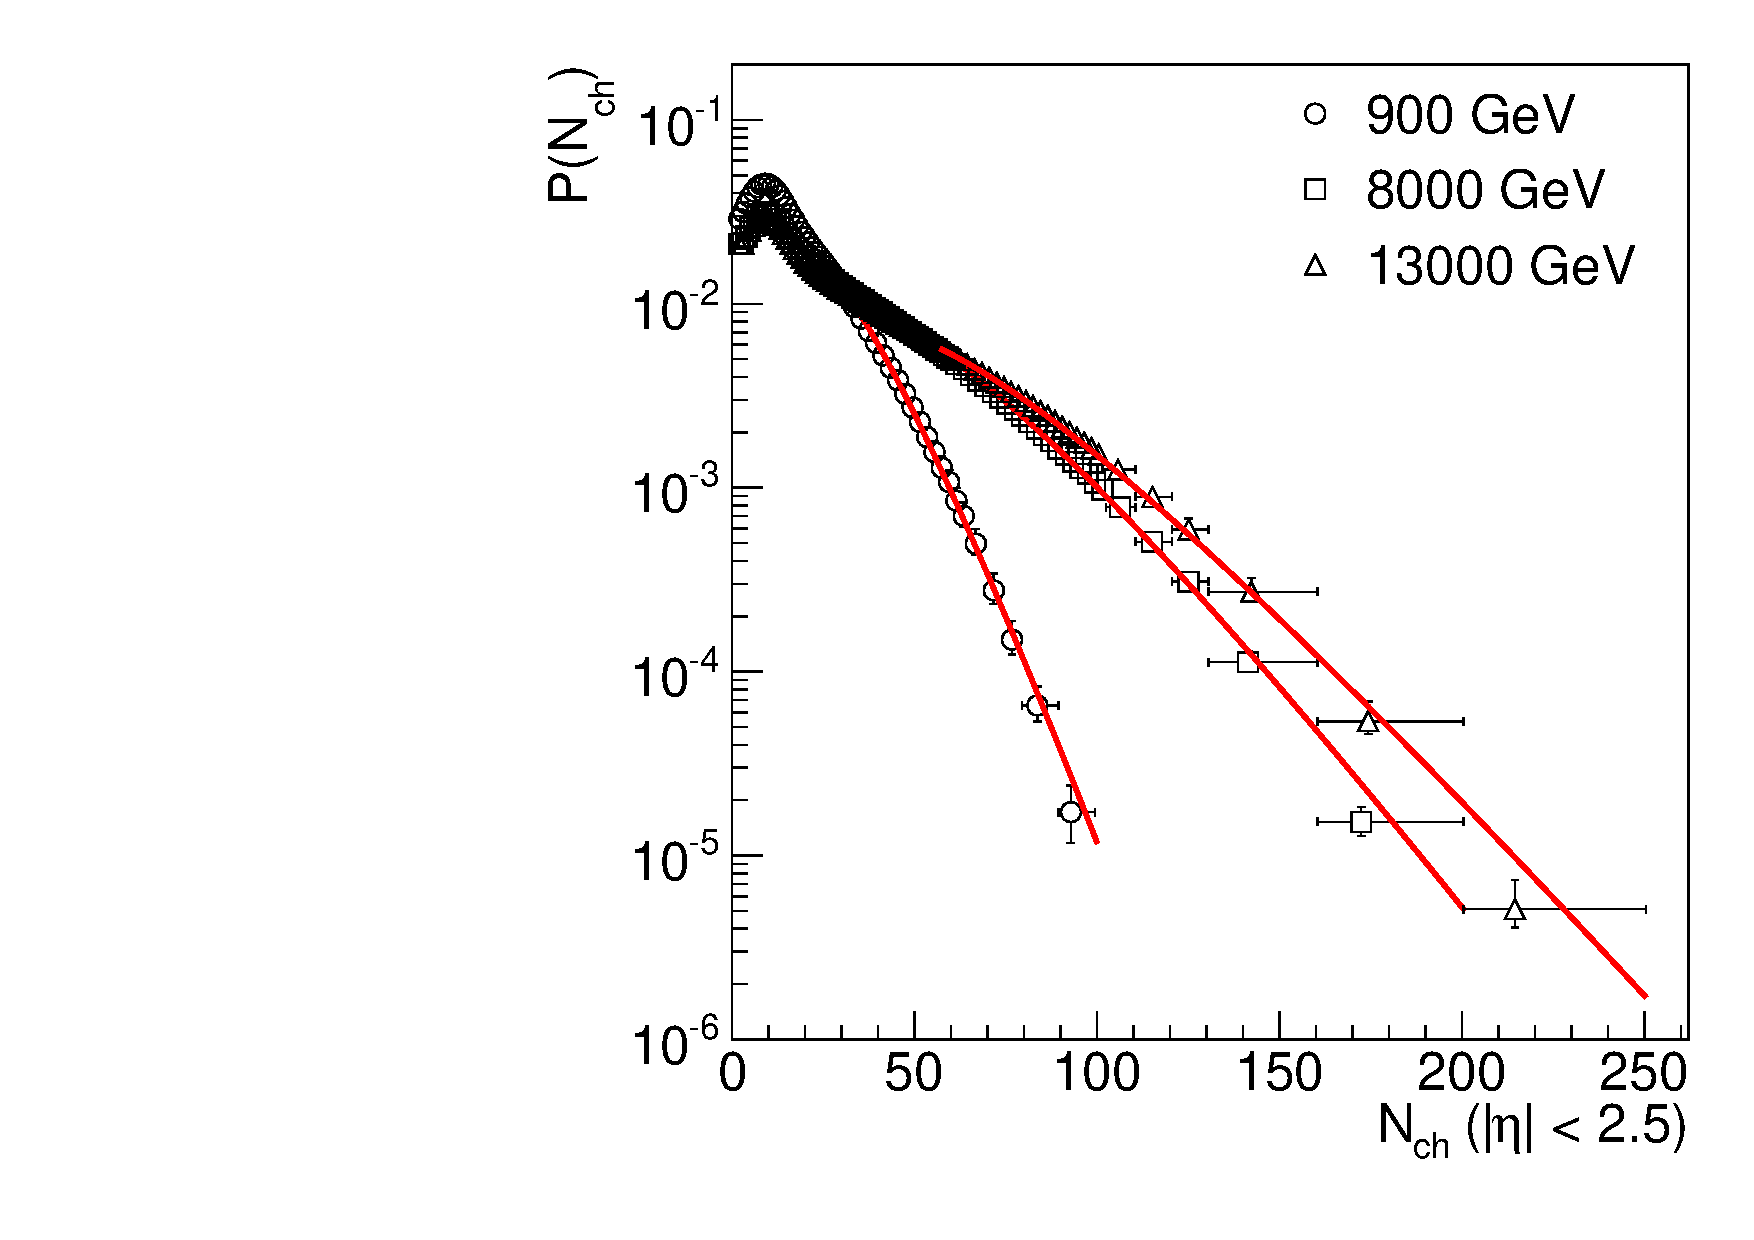
\includegraphics[width=0.49\linewidth]{\main/smallsystems/img/mult_data_11.pdf}
\caption{Multiplicity distributions measured by ALICE (left panel) and ATLAS (right panel) overlaid by the fit with a negative binomial distribution.}
\label{fig:smallsystems_mult_data}
\end{figure}

\begin{figure}[ht]
\centering
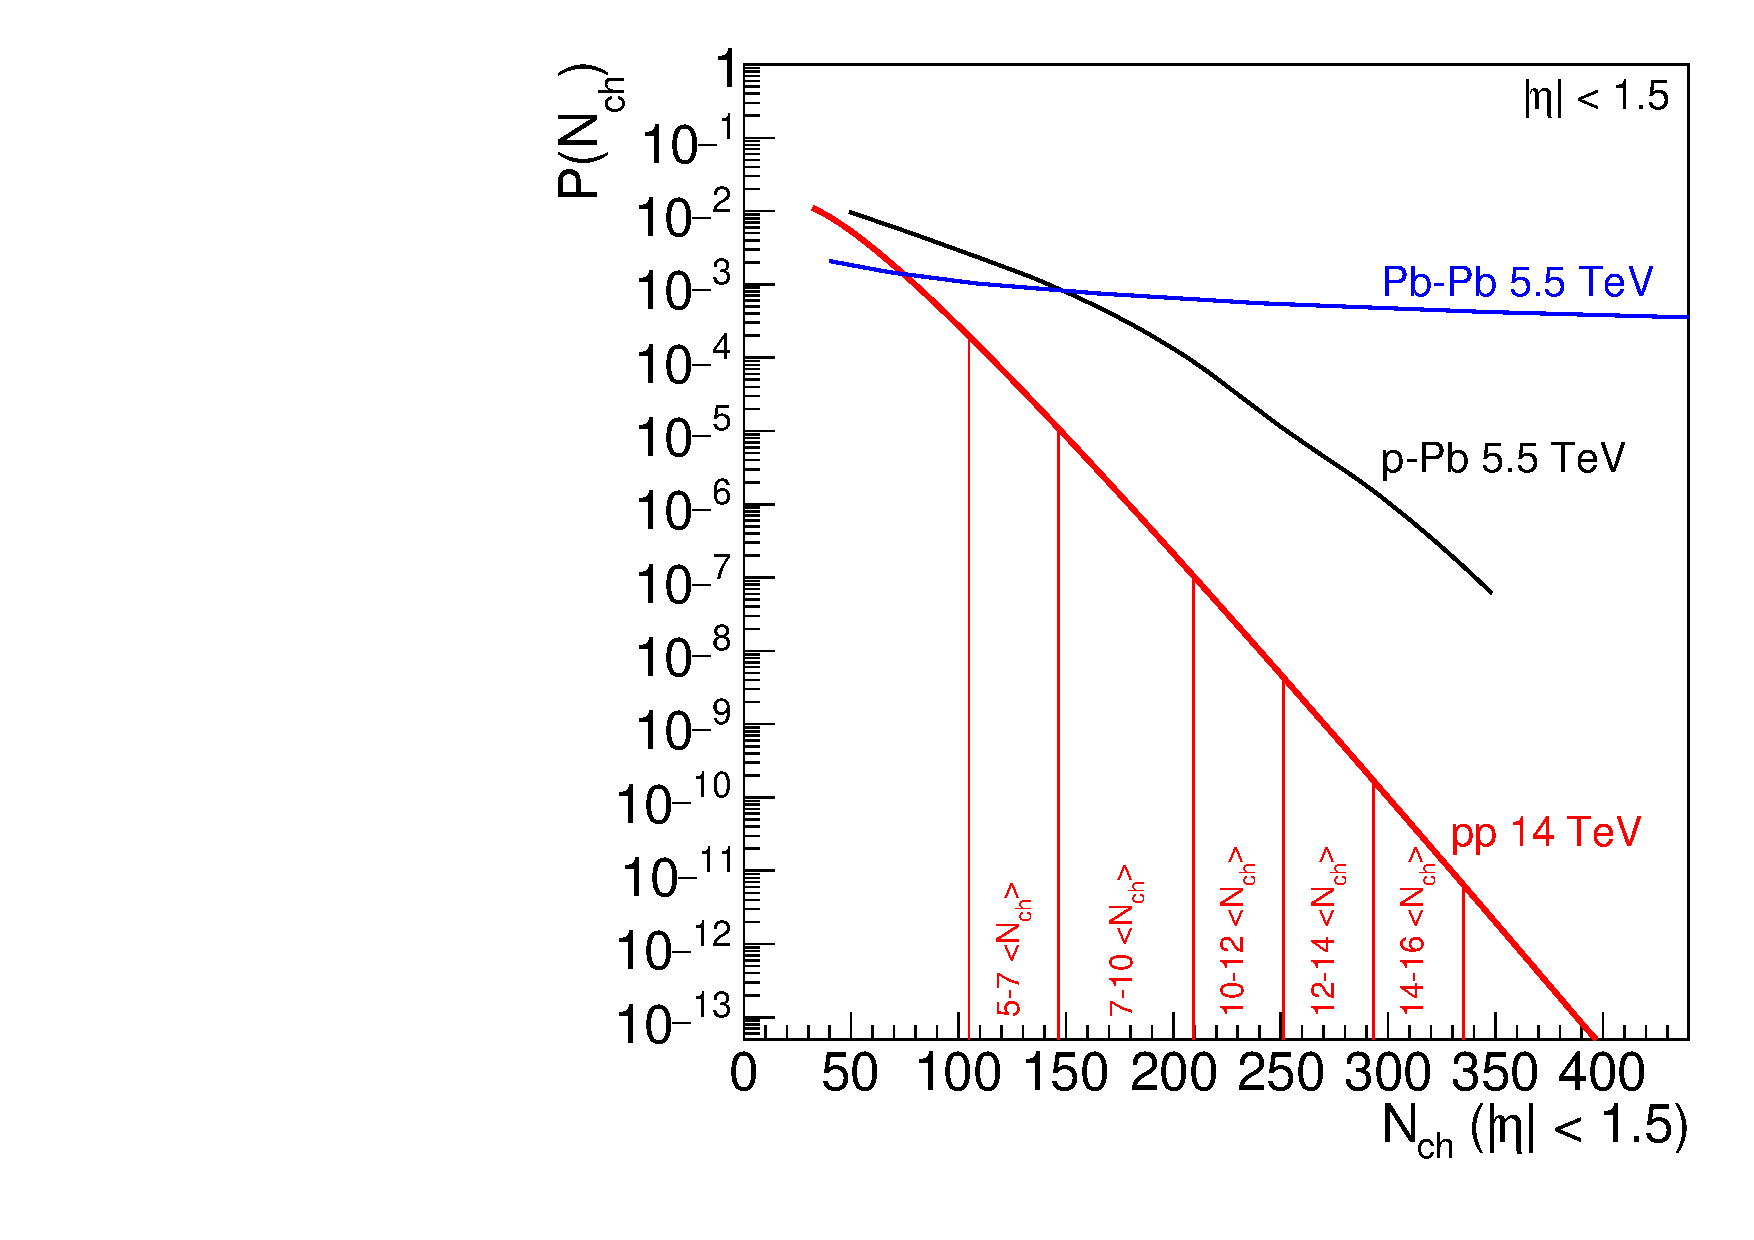
\includegraphics[width=0.32\linewidth]{\main/smallsystems/img/mult_extrapolation_alice.pdf}
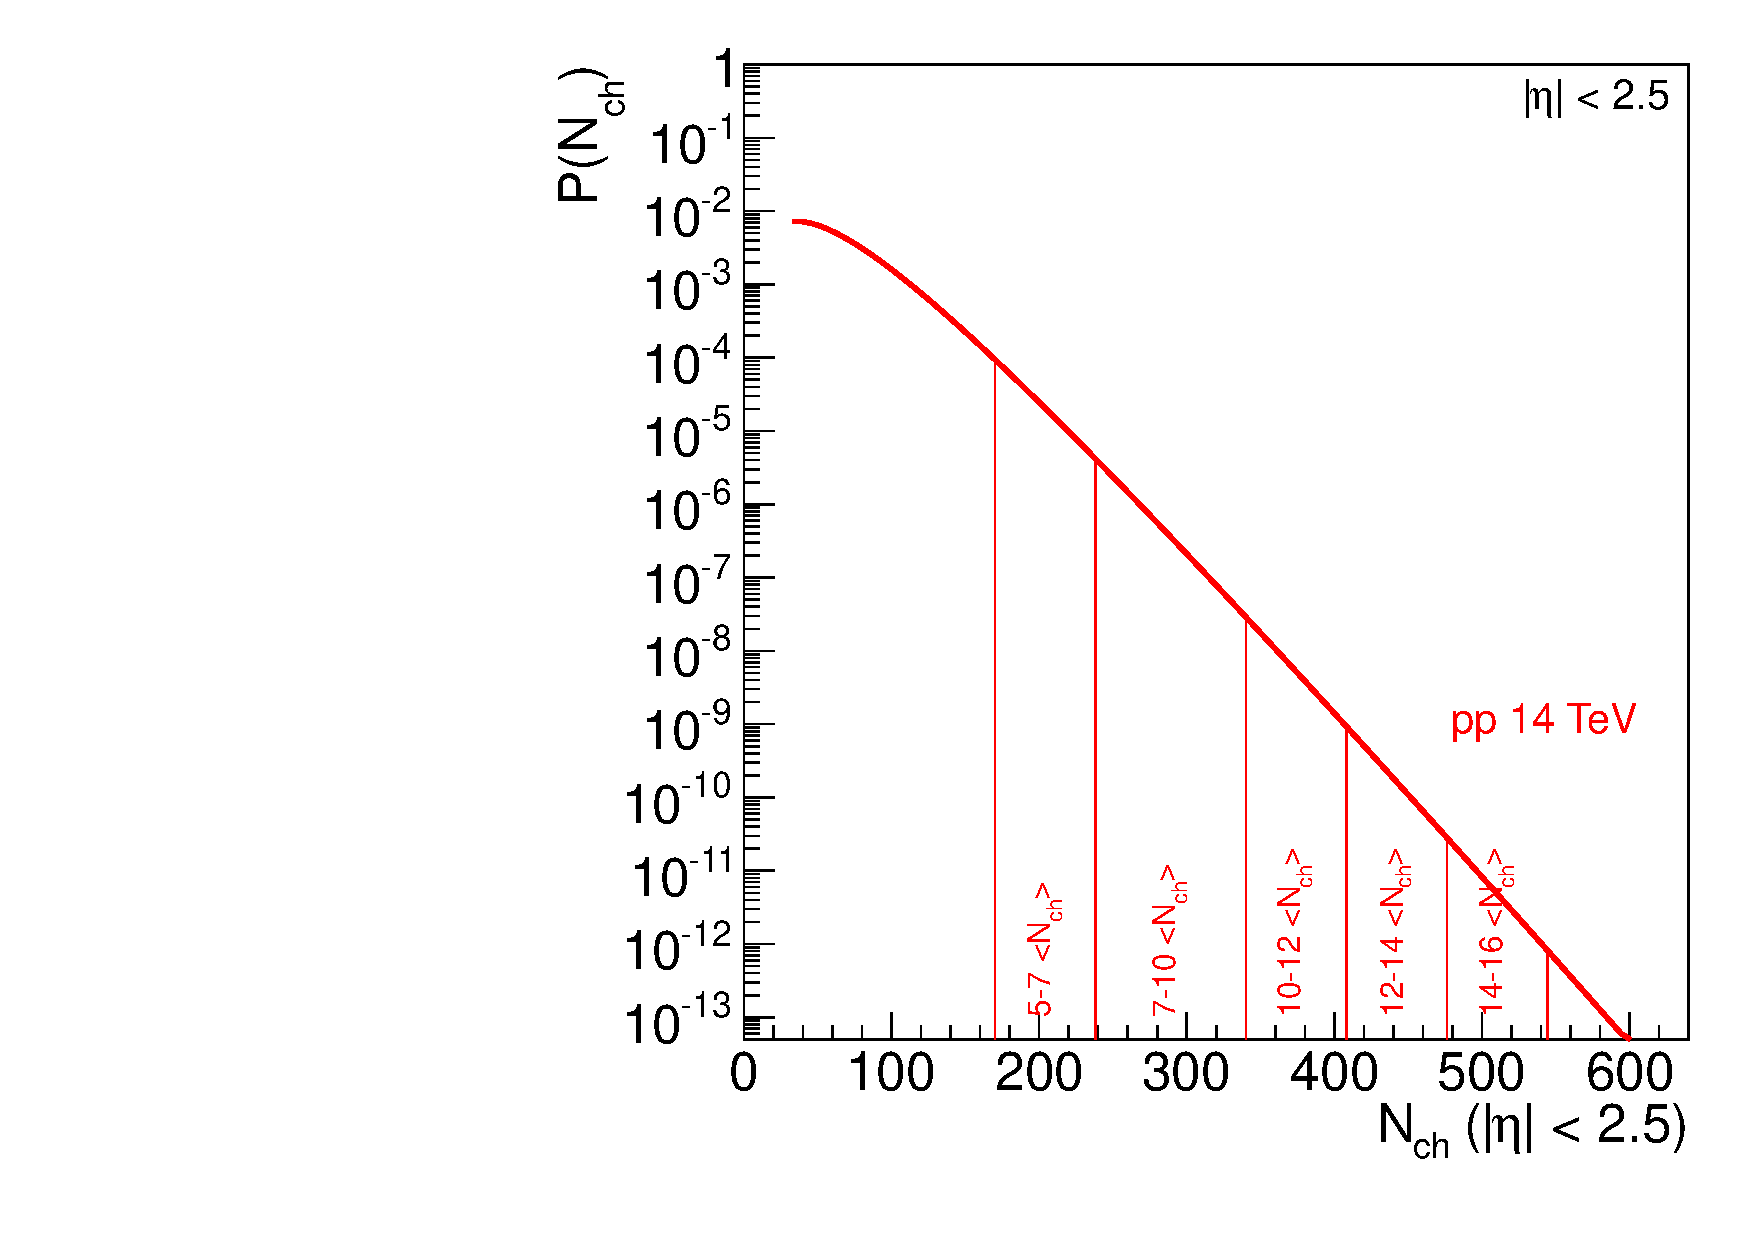
\includegraphics[width=0.32\linewidth]{\main/smallsystems/img/mult_extrapolation_atlas.pdf}
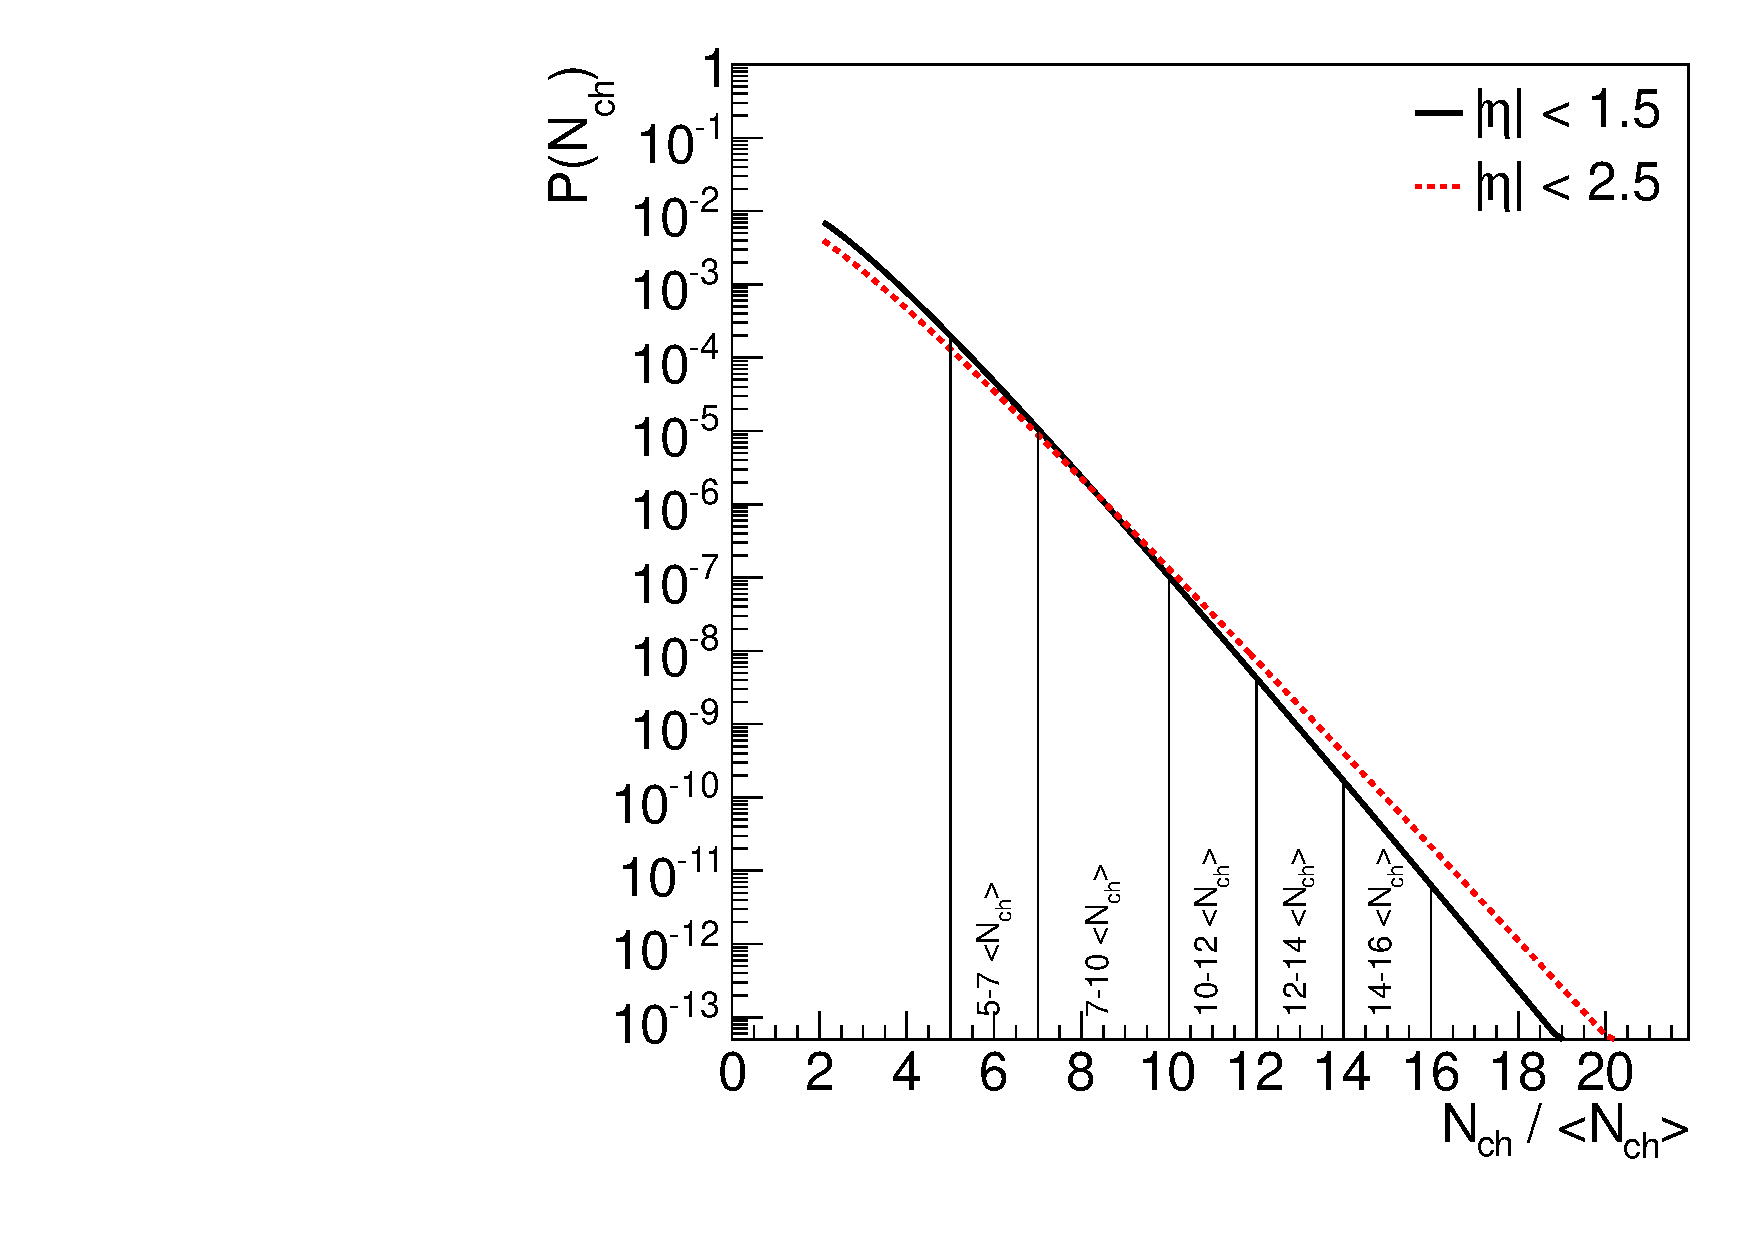
\includegraphics[width=0.32\linewidth]{\main/smallsystems/img/mult_extrapolation_comparison.pdf}
\caption{Extrapolated multiplicity distributions in pp collisions within $|\eta| < 1.5$ (left panel) and $|\eta| < 2.5$ (center panel). The indicated regions are from left to right for 5--7, 7--10, 10--12, 12--14, 14--16 times the average multiplicity. In the left panel the multiplicity distribution of Pb--Pb and p--Pb collisions is also plotted. The right panel compares these two distributions scaled by the average multiplicity. The extrapolation for $|\eta| < 2.5$ turns out to be a bit wider at large multiplicities; therefore the one based on $|\eta| < 1.5$ is used as baseline.}
\label{fig:smallsystems_mult_extrapolation}
\end{figure}

The resulting extrapolated multiplicity distribution for 14~TeV is shown in Fig.~\ref{fig:smallsystems_mult_extrapolation} for the ALICE and ATLAS case. In addition, these are compared scaled by their respective average multiplicities. The agreement is rather good, with some discrepancy in the tail of the distribution. The extrapolation based on the smaller phase space region falls off more quickly with multiplicity, and is therefore used as the more conservative estimate for all extrapolations.

Table~\ref{tab:smallsystems_pp} gives the fraction of cross-section and the number of events in 5 multiplicity classes:  5--7, 7--10, 10--12, 12--14 and 14--16 times the average multiplicity. Table~\ref{tab:smallsystems_pbpb} gives the number of events of bins with equivalent multiplicity than commonly measured multiplicity bins in p--Pb and Pb--Pb collisions. For the calculation of the number of events $\sigma_{\rm inel} = \unit[78.4]{mb}$ \cite{Loizides:2017ack} is used. These tables are the key input for the performance figures presented in this section. A high-multiplicity pp program sampling \unit[200]{pb$^{-1}$} is assumed for all experiments.
 
\begin{table}
\centering
\begin{tabular}{c|c|c|c|c}
Range & $\dNdeta$ & Fraction & Events per pb$^{-1}$ & Events in 200~pb$^{-1}$ \\
\hline
5--7 \nch     & 35--49   & 2.4e-03       & 1.9e+08       & 3.7e+10 \\
7--10 \nch    & 49--70   & 1.3e-04       & 1.0e+07       & 2.0e+09 \\
10--12 \nch   & 70--84   & 1.1e-06       & 9.0e+04       & 1.8e+07 \\
12--14 \nch   & 84--98   & 4.7e-08       & 3.7e+03       & 7.3e+05 \\
14--16 \nch   & 98--112  & 1.8e-09       & 1.4e+02       & 2.8e+04 \\
\hline
\end{tabular}
\caption{Number of pp events at 14 TeV in selected multiplicity bins.}
\label{tab:smallsystems_pp}
\end{table}

\begin{table}
\centering
\begin{tabular}{l|c|c|c}
Range & $\dNdeta$ & Events per pb$^{-1}$ & Events in 200~pb$^{-1}$ \\
\hline
0--5\% p--Pb   & 41--56        & 4.9e+07       & 9.8e+09 \\
5--10\% p--Pb  & 34--41        & 1.9e+08       & 3.8e+10 \\
10--20\% p--Pb & 27--34        & 6.6e+08       & 1.3e+11 \\
\hline
60--65\% Pb--Pb    & 98--137       & 1.5e+02       & 3.0e+04 \\
65--70\% Pb--Pb    & 68--98        & 1.6e+05       & 3.1e+07 \\ 
70--75\% Pb--Pb    & 45--68        & 2.1e+07       & 4.2e+09 \\
75--80\% Pb--Pb    & 29--45        & 5.9e+08       & 1.2e+11 \\
\hline
\end{tabular}
\caption{Number of events in pp collisions at 14 TeV sliced in equivalent multiplicity bins as in p--Pb and Pb--Pb collisions.}
\label{tab:smallsystems_pbpb}
\end{table}

\todo{plot on energy density}

\subsubsection{Particle Correlations}

The measurements of two-particle correlations and higher-order cumulants have produced the initial observations of collectivity in small systems. In pp collisions, two distinct regions are of interest at HL-LHC: the high-multiplicity tail and the low-multiplicity regions. 

In pPb collisions, ...

The 4-particle cumulant is calculated for the third-order harmonics. Figure~\ref{fig:smallsystems_corr_cumulants} compares the $c_3\{4\}$ values between the published and the projected results, for $pp$ and $p$+Pb. In order to remove the non-flow contributions, 3-subevent method is applied. In the $pp$ collisions, with the data collected in Run 2, the statistical uncertainties are large and the $c_3\{4\}$ values are systematically consistent with zero in most $N_{ch}$ ranges. While in large systems, significant non-zero $c_3\{4\}$ has been measured, which reflects the fluctuation of triangle flow. Whether similar behavior is observed in small systems still needs to be confirmed. The increase in luminosity in Run 3 and Run 4 provides a great opportunity to measure $c_3\{4\}$ in $pp$ with high precision: the statistics are sufficient to measure down to $1.5\%$ $v_3\{4\}$ in the high multiplicity region. Similarly, in the $p$+Pb collision, the current result shows that $c_3\{4\}$ is consistent with zero, but increased statistics will help to detect potential non-zero $c_3\{4\}$ down to $1.5\%$ in most multiplicity ranges.

\begin{figure}[ht]
\centering
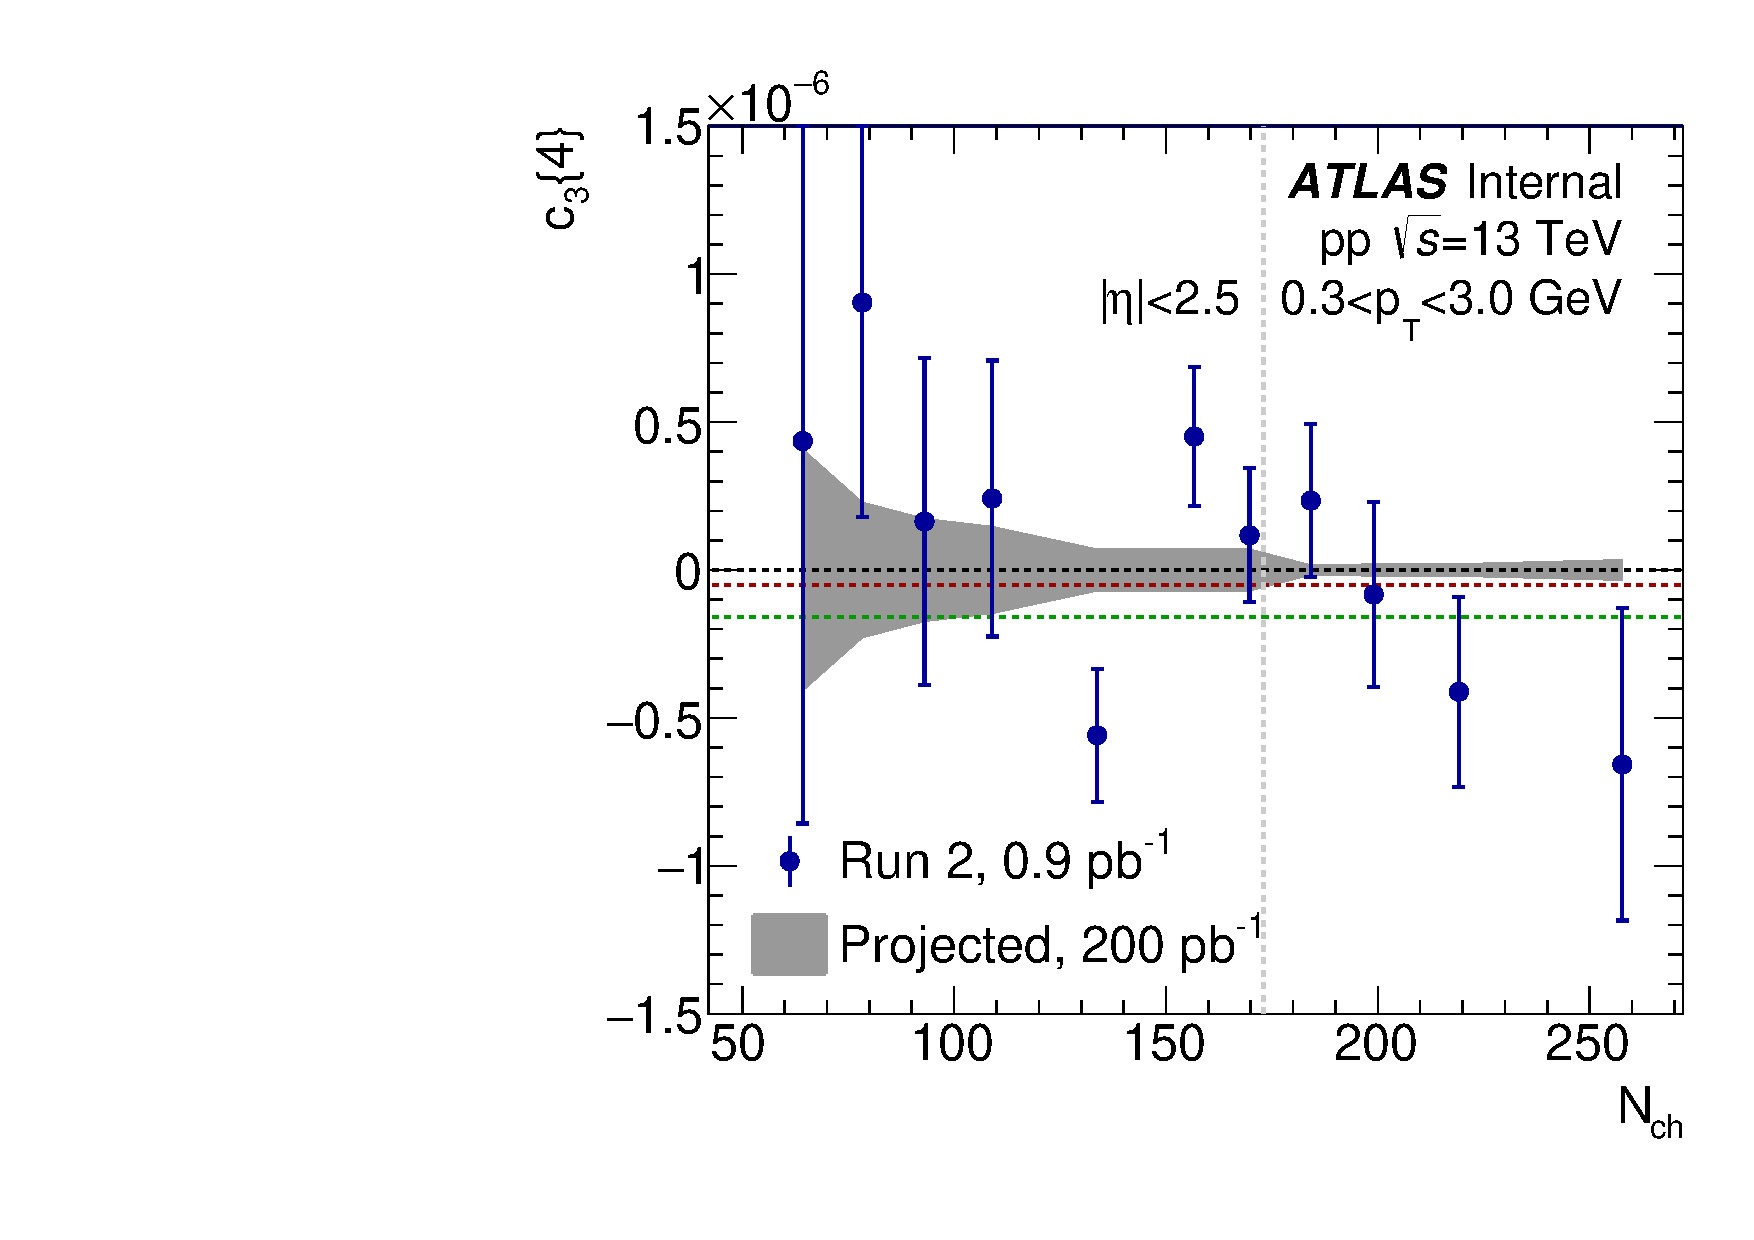
\includegraphics[width=.45\linewidth]{\main/smallsystems/img/c_3_4_pp.pdf}
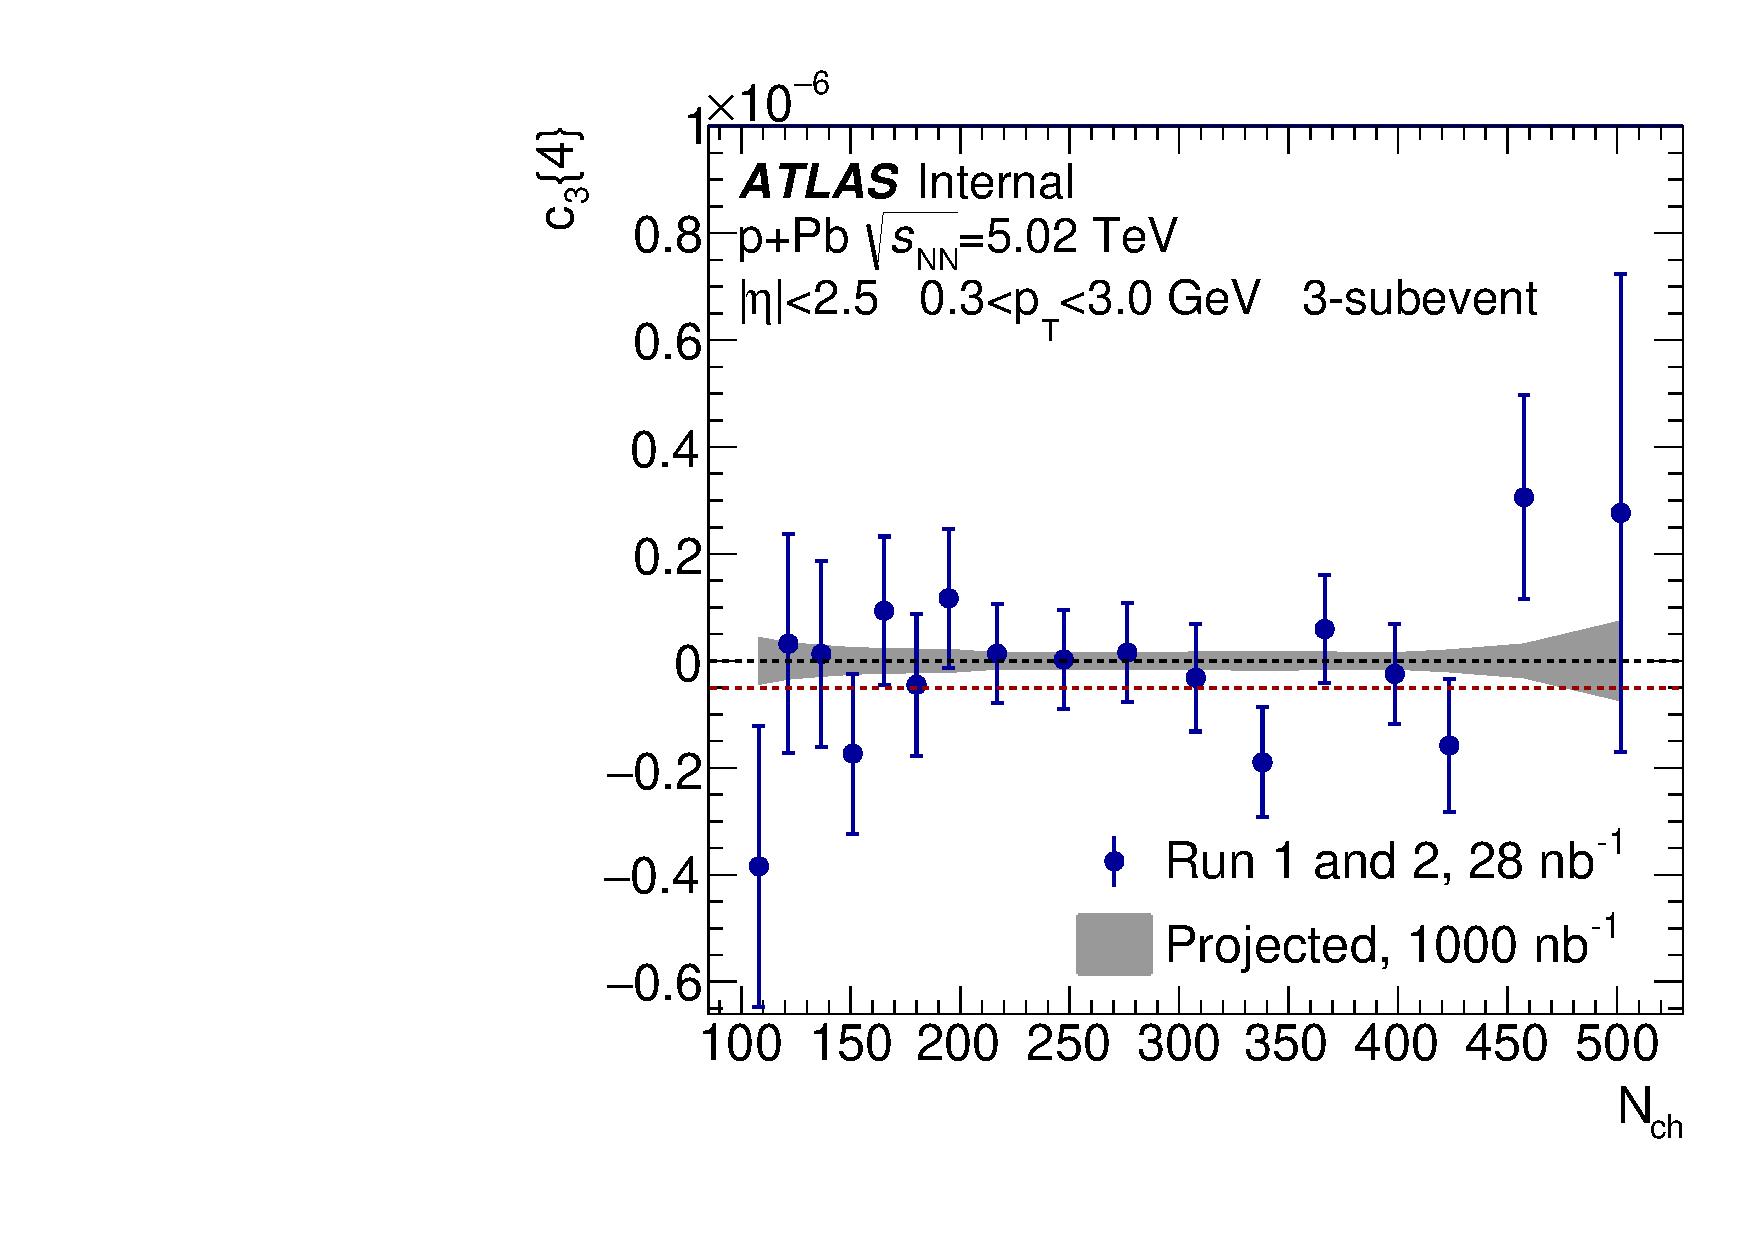
\includegraphics[width=.45\linewidth]{\main/smallsystems/img/c_3_4_pPb.pdf}
%\includegraphics[draft]{img/corr_cumulants.pdf}
\caption{4-particle cumulants $c_3\{4\}$ with 3-subevent method for $pp$ (left) and $p$+Pb (right) as a function of $N_{ch}$. Only statistical uncertainties are shown in the figure and the gray band represents the projected statistical uncertainty, with $c_3\{4\}$ assumed to be zero. The red and green dash lines represent $1.5\%$ and $2.0\%$ $v_3\{4\}$ signal respectively.}
\label{fig:smallsystems_corr_cumulants}
\end{figure}

\begin{figure}[ht]
\centering
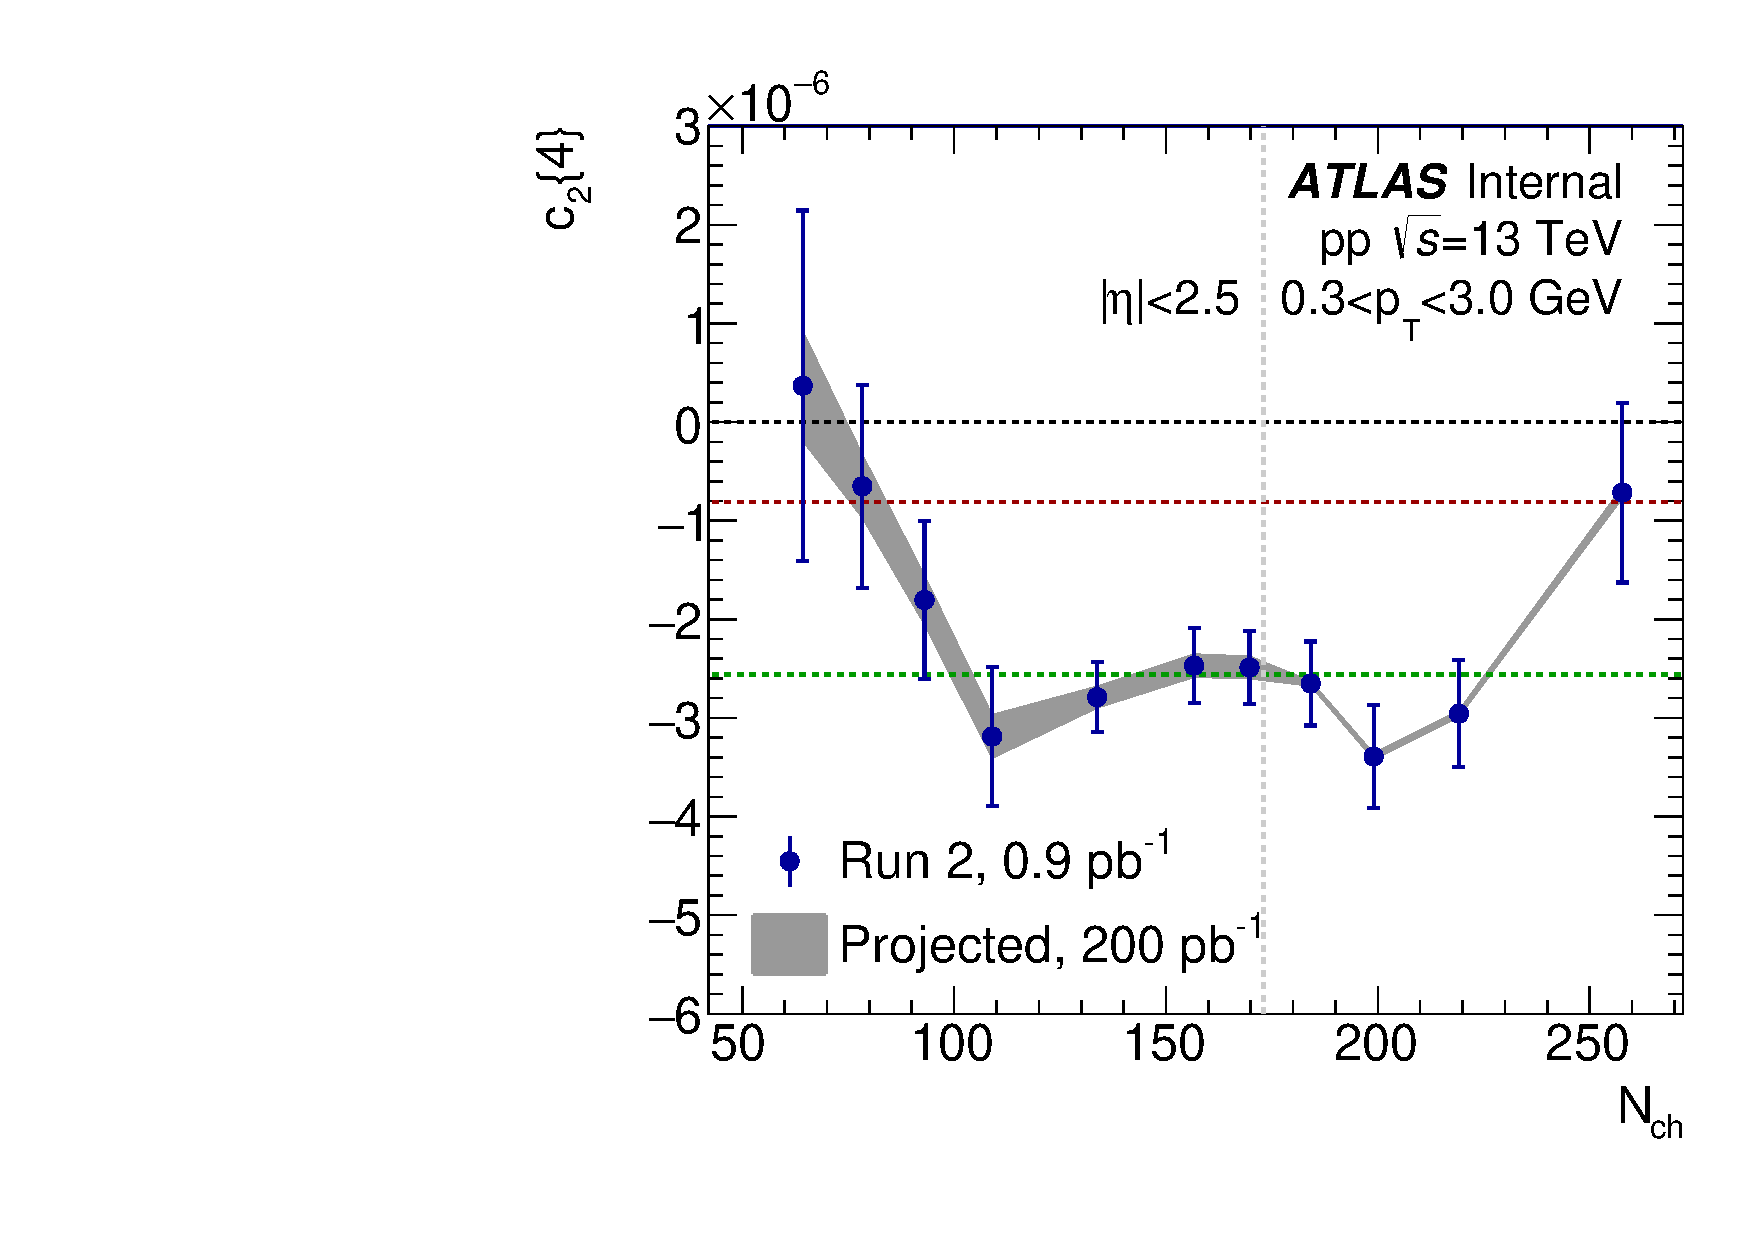
\includegraphics[width=.45\linewidth]{\main/smallsystems/img/c_2_4_pp.pdf}
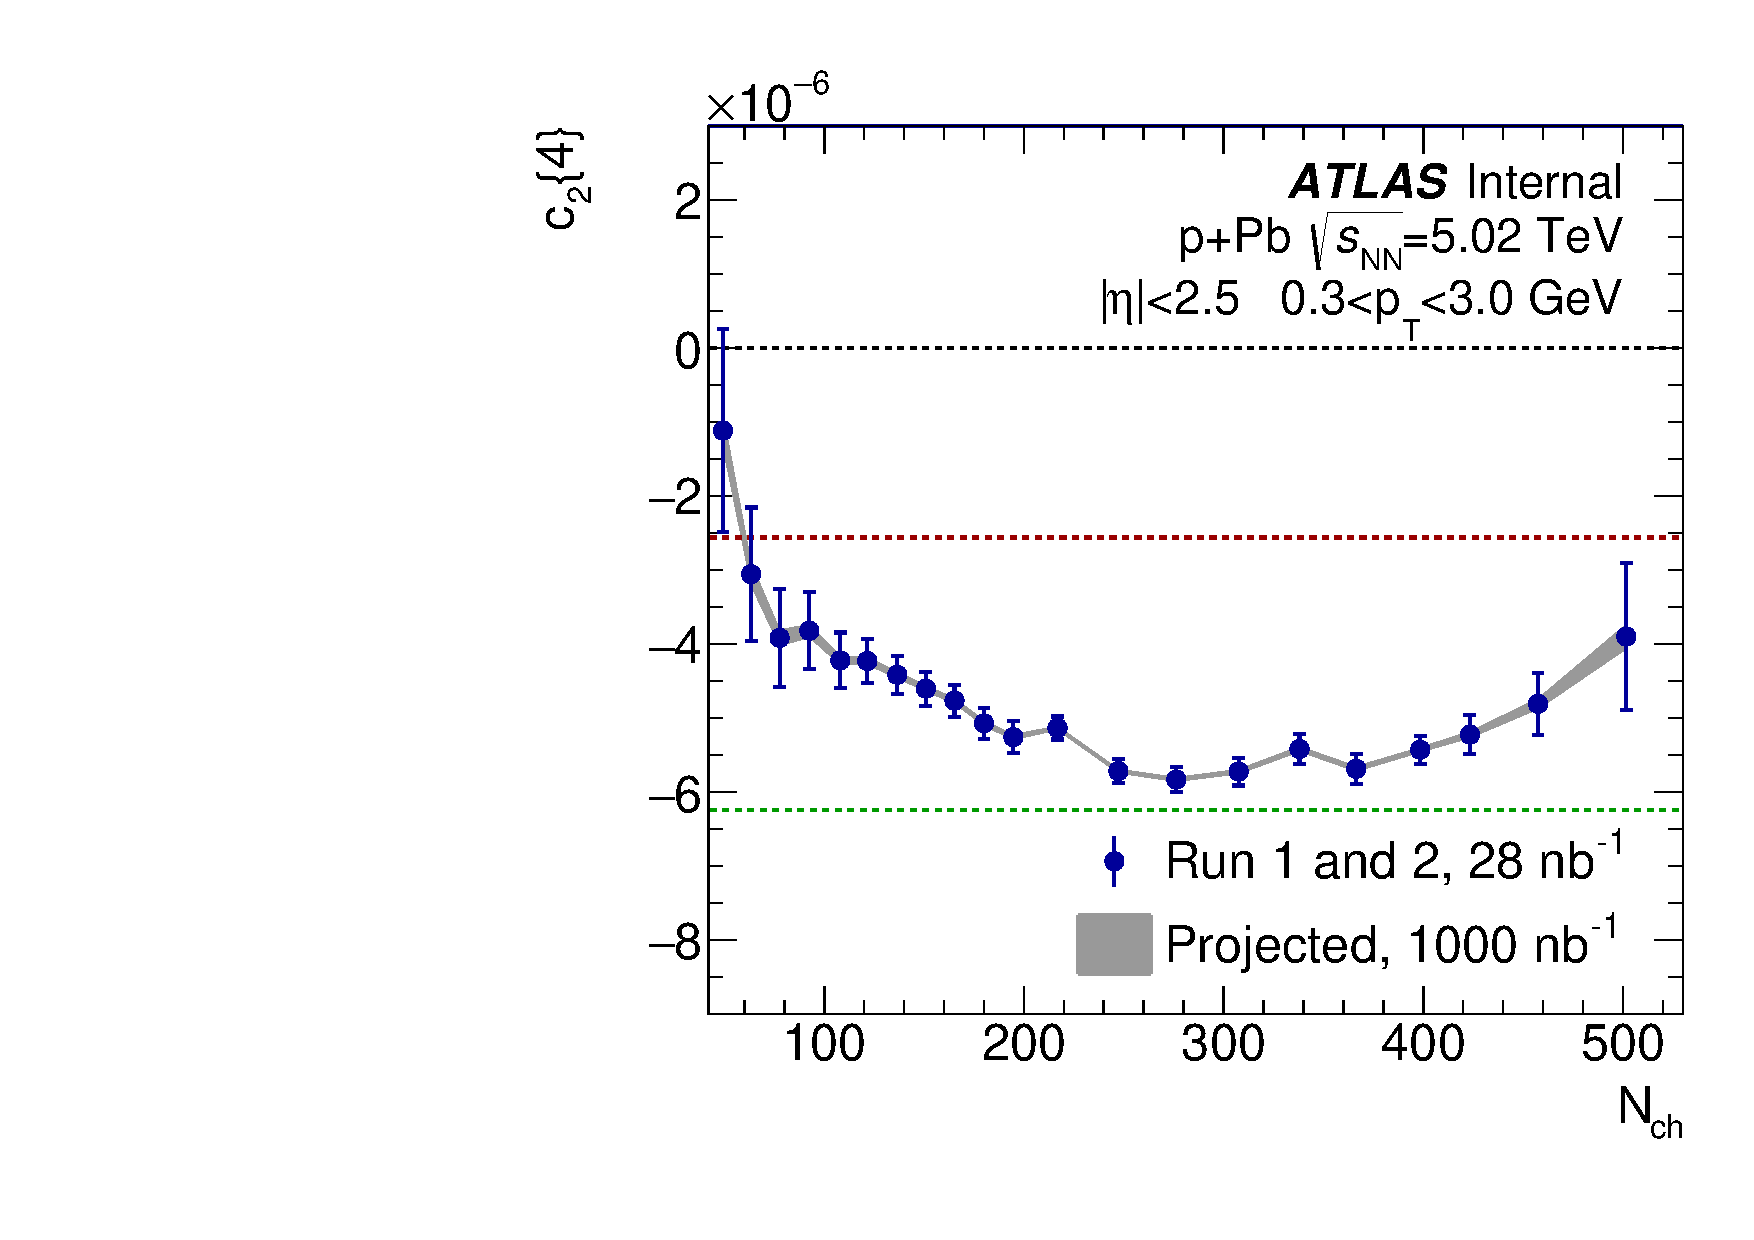
\includegraphics[width=.45\linewidth]{\main/smallsystems/img/c_2_4_pPb.pdf}
%\includegraphics[draft]{img/corr_cumulants.pdf}
\caption{4-particle cumulants $c_2\{4\}$ with 3-subevent method for $pp$ (left) and $p$+Pb (right) as a function of $N_{ch}$. Only statistical uncertainties are shown in the figure and the gray band represents the projected statistical uncertainty. The red and green dash lines represent $3\%$ and $4\%$ $v_2\{4\}$ signals for $pp$, and $4\%$ and $5\%$ $v_2\{4\}$ signals for $p$+Pb.}
\label{fig:smallsystems_corr_cumulants_v2}
\end{figure}



\begin{figure}[ht]
\centering
\includegraphics[draft]{\main/smallsystems/img/corr_symmetriccumulants.pdf}
%\includegraphics[draft]{img/corr_symmetriccumulants.pdf}
\caption{Symmetric cumulants extracted with and without applying subevents for pp (left) and pPb (right) as a function of Nch. CMS.}
\label{fig:smallsystems_corr_symmetriccumulants}
\end{figure}

\begin{figure}[ht]
\centering
\includegraphics[draft]{\main/smallsystems/img/corr_cumulants_pid.pdf}
%\includegraphics[draft]{img/corr_cumulants_pid.pdf}

\caption{Particle identified $v_n$ (TODO only v2?) coefficients for pi, K, p (pp, ALICE), D mesons (pp, CMS), J/Psi (pp, pPb, ALICE, CMS) as a function of pT. Note that the multiplicity ranges are different for the different estimates. TODO: Plot may be messy and may need splitting in several panels.}
\label{fig:smallsystems_corr_cumulants_pid}
\end{figure}

\subsubsection{Event-by-event fluctuations of elliptic flow $\rm{P}(v_{2})$}

The $v_n$ measurements fluctuate on an event by event basis as no two nuclei have identical parton distribution. Probability denisity distribution, $\rm{P}(v_n)$ is closely related to event-by-event fluctuations of the eccentricities, $\rm{P}(\varepsilon_{n})$. As a result,  
study of probability density distribution, $\rm{P}(v_n)$,  provides more information about the initial condition and the final state dynamics of the medium. Models predict a semi-gaussian distribution of $\rm{P}(v_{n})$ in large systems, while, in small systems the shape is predicted to be closer to a gaussian. Figure \ref{fig:smallsystems_corr_pvn} presents the measurement of $\rm{P}(v_{2})$ in $60-65\%$ centrality Pb--Pb collisions at $\sqrt{s_{\rm{NN}}} = $ 2.76 TeV recorded by ATLAS experiment. The results have been projected to the LHC run 3 and run 4 data with the same multiplicity range of pp collisions at $\sqrt{s} = 14$ TeV. 

\begin{figure}[ht]
\centering
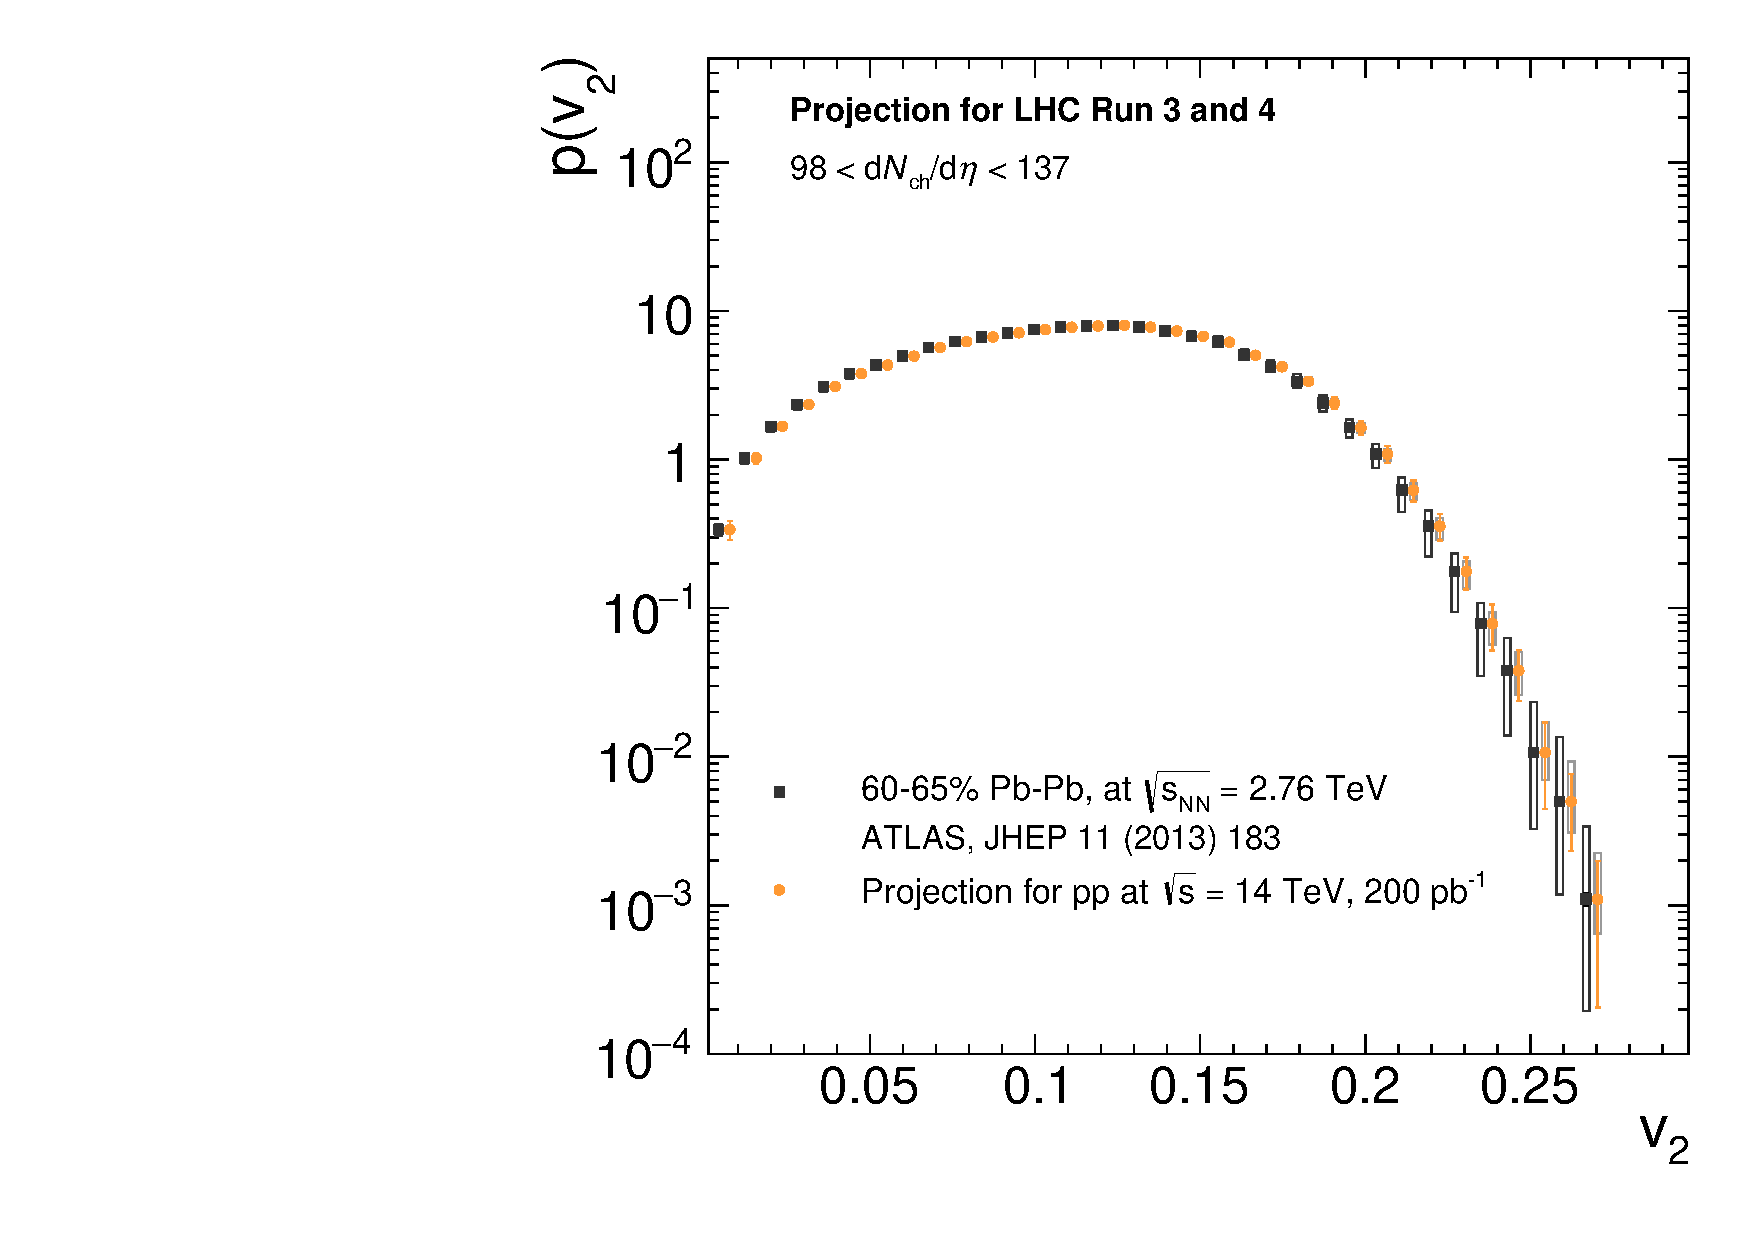
\includegraphics[width=.49\linewidth]{\main/smallsystems/img/ebye_v2_60-65_276TeVppprojection.pdf}

\caption{Projection of the measurement of the probability distribution of $v_2$ in pp collisions. To illustrate the reach the same signal as in Pb--Pb is assumed. The projection is for the equivalent pp multiplicity (circles) to 60--65\% centrality in Pb--Pb collisions (squares).}
\label{fig:smallsystems_corr_pvn}
\end{figure}

\subsubsection{Strangeness Enhancement}

\begin{figure}[ht]
\centering
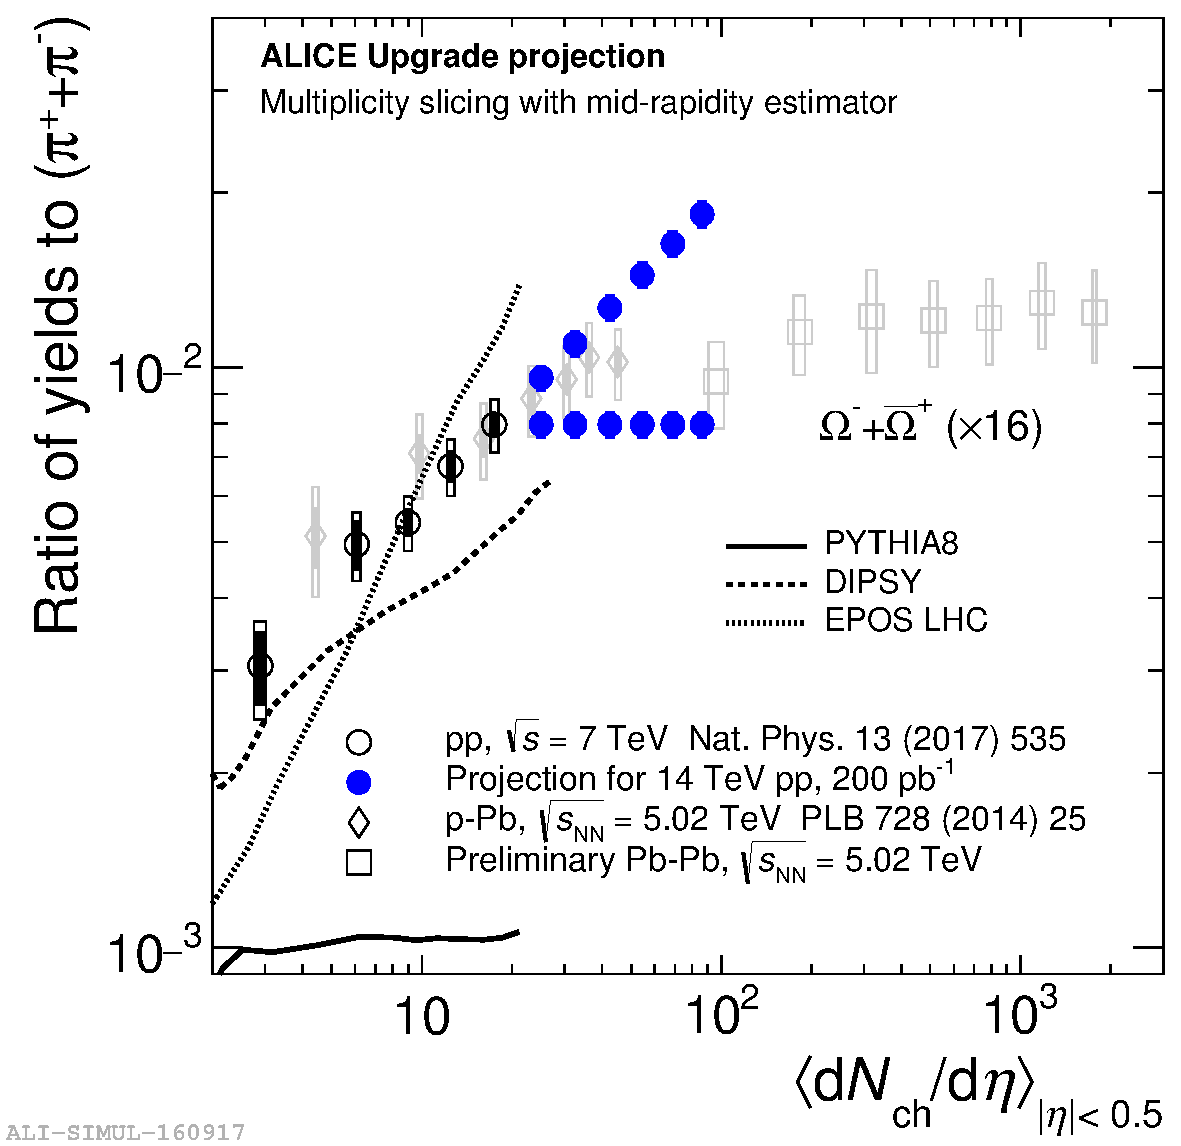
\includegraphics[width=0.49\linewidth]{\main/smallsystems/img/strangeness_omegapi.pdf}

\caption{$\Omega/\pi$ ratio as a function of $\nch$ for pp, p--Pb, and Pb--Pb collisions. The existing data (from Ref.~\cite{ALICE:2017jyt}) is shown in open black symbols, the extrapolation for pp collision is denoted by blue filled circles.}
\label{fig:smallsystems_strangeness_omega_pi}
\end{figure}

\subsubsection{Energy Loss}

Narrative: 
- Existing pA eloss measurements (ALICE, ATLAS, CMS) show limit of maximal few percent quenching. In conclusion, RpA is not a good observable
- Produce estimates for a) h-jet (a la ALICE), b) gamma-jet or Z-jet (ATLAS/CMS), c) jet substructure
- Produce these for pA and pp
- For pp, see if high mu sample can be also used for something. In fact it should be made clear where it can be used and where not, as this chapter will be one of the places where a low mu pp program is motivated.

\begin{figure}[ht]
\centering
\includegraphics[draft]{\main/smallsystems/img/energyloss_hjet.pdf}
%\includegraphics[draft]{img/energyloss_hjet.pdf}
\caption{Modification of jet recoil yields extracted from hadron-jet correlations for pp collisions (left) and p-Pb collisions (right). Delta-recoil ratio vs. pT.}
\label{fig:smallsystems_energyloss_hjet}
\end{figure}

\begin{figure}[ht]
\centering
\includegraphics[draft]{\main/smallsystems/img/energyloss_Zjet.pdf}
%\includegraphics[draft]{img/energyloss_Zjet.pdf}

\caption{Z-jet correlations in pp (left panel) and p-Pb collisions (right panel). 1/N dN/dxZj vs xZj.}
\label{fig:smallsystems_energyloss_Zjet}
\end{figure}

\subsubsection{Thermal Radiation}

\begin{figure}[ht]
\centering
\includegraphics[draft]{\main/smallsystems/img/thermal_radiation.pdf}
\caption{Thermal dileptons. Left panel: dN/Mee vs. Mee Example. Right panel: sensitivity as a function of Lint (pp, pPb) [expected signal is too uncertain].}
\label{fig:smallsystems_thermal_radition}
\end{figure}

\subsection{Data-taking strategy}

% High multiplicity triggering, pile up, MB sample
% pp
%   ALICE: additional several month pp program
%   ATLAS/CMS: special runs (mu~1) or special conditions at end of fill
%   LHCb: either in nominal (mu~5) or special running
%   HM sample: 200 pb-1 pp (per experiment)
%   How much MB for low-multiplicity questions?
% p-Pb scheduled run
%   1000-2000 nb-1

\subsection{Summary}

\clearpage

\bibliographystyle{report}   % Remember we use title in the biblio
\bibliography{bib/section}

\end{document}
